\documentclass[11pt,a4paper]{article}
\usepackage[utf8]{inputenc}
\usepackage[T1]{fontenc}
\usepackage{amsmath,amsfonts,amssymb}
\usepackage{graphicx}
\usepackage{hyperref}
\usepackage{listings}
\usepackage{xcolor}
\usepackage{tikz}
\usepackage{pgfplots}
\usepackage{pgfgantt}
\usepackage[margin=0.9in,headheight=15pt]{geometry}
\usepackage{float}
\usepackage{booktabs}
\usepackage{multirow}
\usepackage{array}
\usepackage{fancyhdr}
\usepackage{lastpage}
\usepackage{titlesec}
\usepackage{enumitem}
\usepackage{tcolorbox}
\usepackage{colortbl}
\usepackage{subcaption}

\pgfplotsset{compat=1.17}
\usetikzlibrary{arrows.meta,positioning,shapes.geometric,calc,decorations.markings,patterns,shadows}
% pie chart drawn manually with tikz

% ── Color palette ──
\definecolor{qblue}{HTML}{0066CC}
\definecolor{qgold}{HTML}{D4A017}
\definecolor{qdark}{HTML}{1A1A2E}
\definecolor{qlight}{HTML}{E8F4FD}
\definecolor{qgreen}{HTML}{27AE60}
\definecolor{qred}{HTML}{E74C3C}
\definecolor{qpurple}{HTML}{8E44AD}
\definecolor{qorange}{HTML}{E67E22}
\definecolor{qcyan}{HTML}{00BCD4}
\definecolor{qteal}{HTML}{009688}
\definecolor{backcolour}{HTML}{F7F9FC}
\definecolor{critcolor}{HTML}{FDEDEC}
\definecolor{featcolor}{HTML}{EBF5FB}

% ── Code listing style ──
\lstdefinestyle{mystyle}{
    backgroundcolor=\color{backcolour},
    commentstyle=\color{qgreen},
    keywordstyle=\color{qblue}\bfseries,
    numberstyle=\tiny\color{gray},
    stringstyle=\color{qpurple},
    basicstyle=\ttfamily\scriptsize,
    breaklines=true,
    captionpos=b,
    keepspaces=true,
    numbers=left,
    numbersep=5pt,
    tabsize=2
}
\lstset{style=mystyle}

% ── Header/Footer ──
\pagestyle{fancy}
\fancyhf{}
\rhead{\textcolor{gray}{\small Quillon Project Report v3.0}}
\lhead{\textcolor{gray}{\small February--March 2026}}
\cfoot{\textcolor{gray}{\small Page \thepage\ of \pageref{LastPage}}}
\renewcommand{\headrulewidth}{0.4pt}
\renewcommand{\footrulewidth}{0.2pt}

% ── Section formatting ──
\titleformat{\section}{\Large\bfseries\color{qblue}}{\thesection}{1em}{}[\vspace{-0.5em}\textcolor{qblue}{\rule{\textwidth}{0.8pt}}]
\titleformat{\subsection}{\large\bfseries\color{qdark}}{\thesubsection}{0.8em}{}

% ── Custom environments ──
\newtcolorbox{criticalbox}{colback=critcolor,colframe=qred,title=\textbf{Critical Fix},fonttitle=\color{white},coltitle=white,colbacktitle=qred}
\newtcolorbox{featurebox}{colback=featcolor,colframe=qblue,title=\textbf{Feature Highlight},fonttitle=\color{white},coltitle=white,colbacktitle=qblue}
\newtcolorbox{metricbox}{colback=qlight,colframe=qcyan,boxrule=0.5pt}

\hypersetup{
    colorlinks=true,
    linkcolor=qblue,
    urlcolor=qpurple,
    citecolor=qgreen
}

% ════════════════════════════════════════════════════════════════════
\title{%
\vspace{-1cm}
{\Huge\bfseries\textcolor{qblue}{Quillon}}\\[0.3cm]
{\LARGE\textcolor{qdark}{Project Development Report}}\\[0.2cm]
{\Large v3.0 --- February--March 2026}\\[0.5cm]
\textcolor{qgold}{\rule{0.6\textwidth}{1.5pt}}
}
\author{%
Quillon Development Team\\
\texttt{contact@quillon.xyz}\\[0.3cm]
\textit{Covering: February 1 -- March 28, 2026}
}
\date{}

\begin{document}
\maketitle
\thispagestyle{fancy}

% ════════════════════════════════════════════════════════════════════
\begin{abstract}
\noindent
This report documents the development of the Quillon quantum-resistant blockchain system during the period February 1 through March 28, 2026. Over 57 days and 153 commits, the project advanced from mainnet genesis launch through 25 production releases (v7.4.1 to v10.2.1), deployed four production bootstrap nodes across three continents, fixed 10 critical production bugs, launched the Crown \& Ash on-chain grand strategy game, achieved 7~GH/s network hashrate in 31 days, and survived peer review from professional cryptographers on the metzdowd cryptography mailing list. The codebase grew to 754,442 lines of Rust across 89 crates, supported by 315+ test files and a zero-downtime rolling deployment pipeline. This report presents the technical architecture, development timeline, performance metrics, and lessons learned.
\end{abstract}

\vspace{0.3cm}
\noindent\textbf{Terminology.}
\textit{Quillon} --- the blockchain protocol and network.
\textit{QUG} --- Quillon's native token (21M max supply).
\textit{Crown \& Ash} --- deterministic medieval grand strategy game running on-chain via WASM.
\textit{DAG-Knight} --- Quillon's directed acyclic graph consensus algorithm with BFT finality.
\textit{q-flux} --- custom high-performance reverse proxy built for the Epsilon supernode.
\textit{VDF} --- Verifiable Delay Function, a sequential computation that cannot be parallelized.

\tableofcontents
\newpage

% ════════════════════════════════════════════════════════════════════
\section{Executive Summary}

\begin{metricbox}
\centering
\begin{tabular}{cccc}
\textbf{\textcolor{qblue}{\Large 754,442}} & \textbf{\textcolor{qgreen}{\Large 153}} & \textbf{\textcolor{qpurple}{\Large 89}} & \textbf{\textcolor{qorange}{\Large 25}} \\
Lines of Rust & Commits & Crates & Releases \\[0.3cm]
\textbf{\textcolor{qred}{\Large 10}} & \textbf{\textcolor{qteal}{\Large 7 GH/s}} & \textbf{\textcolor{qgold}{\Large 11.8M}} & \textbf{\textcolor{qblue}{\Large 4}} \\
Critical Bugs Fixed & Network Hashrate & Block Height & Bootstrap Nodes \\
\end{tabular}
\end{metricbox}

\vspace{0.5cm}

The February--March 2026 development cycle represents the most intensive period in the project's history. Starting from mainnet genesis on February 19, the team:

\begin{enumerate}[leftmargin=*]
    \item \textbf{Launched mainnet-genesis} with a 4-year halving emission model (2,625,000 QUG/year Era~0, 21M max supply)
    \item \textbf{Scaled from 1 to 4 bootstrap nodes} (Beta, Gamma, Delta, Epsilon) with zero-downtime rolling deployments
    \item \textbf{Built q-flux}, a high-performance reverse proxy replacing nginx on the 10Gbit Epsilon supernode
    \item \textbf{Shipped GPU mining} with OpenCL BLAKE3+VDF achieving 68.7~MH/s per GTX~1080~Ti ($229\times$ CPU speedup)
    \item \textbf{Launched Crown \& Ash}, a deterministic medieval grand strategy game running entirely on-chain via WASM
    \item \textbf{Survived peer review} on the metzdowd cryptography mailing list from 10 professional cryptographers
    \item \textbf{Fixed 10 critical production bugs} including OOM crash-loops, height regression, and balance race conditions
\end{enumerate}

% ════════════════════════════════════════════════════════════════════
\section{Development Timeline}

\subsection{Gantt Chart: 57-Day Development Sprint}

\begin{figure}[H]
\centering
\resizebox{\textwidth}{!}{%
\begin{ganttchart}[
    hgrid,
    vgrid={*{6}{draw=gray!30}},
    x unit=0.38cm,
    y unit chart=0.55cm,
    y unit title=0.65cm,
    title height=1,
    bar height=0.6,
    bar top shift=0.2,
    group peaks height=0.3,
    title label font=\scriptsize\bfseries,
    bar label font=\scriptsize,
    group label font=\scriptsize\bfseries,
    milestone label font=\scriptsize\bfseries\color{qred},
    today=37,
    today label=Today,
    today label font=\tiny\color{qred}\bfseries,
    today rule/.style={draw=qred, ultra thick, dashed},
    bar/.append style={fill=qblue!60},
    bar incomplete/.append style={fill=qblue!20},
    group/.append style={draw=qdark, fill=qdark!80},
    group left shift=0, group right shift=0,
    milestone/.append style={fill=qred, shape=diamond, inner sep=1.5pt}
]{1}{57}

% Title: weeks
\gantttitle{February 2026}{28}
\gantttitle{March 2026}{29} \\
\gantttitlelist{1,...,57}{1} \\

% ── Group: Infrastructure ──
\ganttgroup{Infrastructure \& Ops}{1}{57} \\
\ganttbar{Mainnet Genesis Prep}{1}{18} \\
\ganttmilestone{Genesis Launch (Feb 19)}{19} \\
\ganttbar{HA Deploy Pipeline}{15}{25} \\
\ganttbar{Delta Bootstrap Node}{19}{22} \\
\ganttbar{Epsilon Supernode Setup}{25}{35} \\
\ganttbar{q-flux Reverse Proxy (9 phases)}{30}{48} \\
\ganttbar{Rolling Deploys (v7--v10)}{19}{57} \\

% ── Group: Core Engine ──
\ganttgroup{Core Engine \& Sync}{1}{57} \\
\ganttbar{Height Regression Fix}{19}{21} \\
\ganttbar{RocksDB Memory Capping}{19}{22} \\
\ganttbar{Turbo Sync Optimization}{22}{35} \\
\ganttbar{Block-Pack Semaphore (OOM fix)}{34}{36} \\
\ganttbar{Gossipsub Flood Fix}{38}{40} \\
\ganttbar{Watermark Race Fix}{55}{57} \\

% ── Group: Mining ──
\ganttgroup{Mining System}{20}{57} \\
\ganttbar{CPU Mining Baseline}{20}{28} \\
\ganttbar{OpenCL GPU Backend}{35}{48} \\
\ganttbar{Kernel Cache + Adaptive Sizing}{45}{50} \\
\ganttbar{Multi-GPU + MinerLink QR}{50}{55} \\
\ganttmilestone{68.7 MH/s Achieved}{50} \\

% ── Group: Privacy & PQ ──
\ganttgroup{Privacy \& Post-Quantum}{10}{57} \\
\ganttbar{Tor rustls Migration}{10}{15} \\
\ganttbar{q-log-privacy Crate}{40}{45} \\
\ganttbar{SQIsign FFI Scaffold}{48}{52} \\
\ganttbar{Dilithium5 Integration}{15}{25} \\

% ── Group: Crown & Ash ──
\ganttgroup{Crown \& Ash Game}{40}{57} \\
\ganttbar{Types + Sim Engine}{40}{48} \\
\ganttbar{WASM Plugin Bridge}{46}{50} \\
\ganttbar{REST API + Persistence}{48}{52} \\
\ganttbar{Bevy Client (ECS)}{50}{55} \\
\ganttbar{API Integration + SSE}{55}{57} \\

% ── Group: Frontend ──
\ganttgroup{Frontend \& Mobile}{15}{57} \\
\ganttbar{Quantum Wallet Enhancements}{15}{40} \\
\ganttbar{Mobile Metro Shims + DEX}{42}{50} \\
\ganttbar{Network Power Modal}{50}{55} \\
\ganttbar{Slint Wallet Auto-Update}{35}{45} \\

% ── Group: Academic ──
\ganttgroup{Academic \& Community}{25}{57} \\
\ganttbar{Metzdowd Announcement}{25}{28} \\
\ganttbar{Peer Review Thread}{28}{57} \\
\ganttbar{Scalability Reply (jrzx)}{52}{57} \\
\ganttbar{100 GH/s Growth Plan}{45}{50}

\end{ganttchart}
}
\caption{Development Gantt chart: 57-day mainnet sprint (Feb 1 -- Mar 28, 2026). Red diamond = milestone, dashed line = report date.}
\label{fig:gantt}
\end{figure}

\subsection{Version Release Timeline}

\begin{figure}[H]
\centering
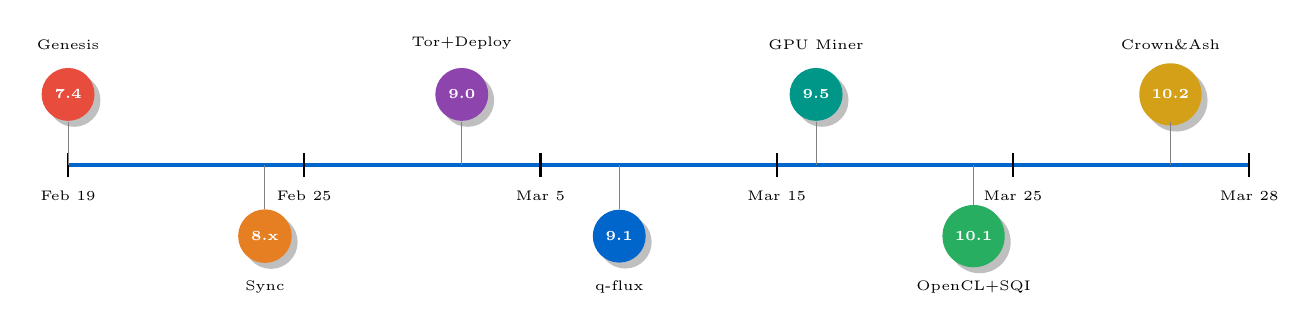
\begin{tikzpicture}[scale=1]
    % Timeline axis
    \draw[ultra thick, qblue] (0,0) -- (15,0);

    % Tick marks and dates
    \foreach \x/\label in {0/Feb 19, 3/Feb 25, 6/Mar 5, 9/Mar 15, 12/Mar 25, 15/Mar 28} {
        \draw[thick] (\x,-0.15) -- (\x,0.15);
        \node[below, font=\tiny] at (\x,-0.2) {\label};
    }

    % Version bubbles (alternating above/below)
    \node[circle, fill=qred, text=white, font=\tiny\bfseries, minimum size=0.55cm, drop shadow] at (0, 0.9) {7.4};
    \node[font=\tiny, above] at (0, 1.35) {Genesis};

    \node[circle, fill=qorange, text=white, font=\tiny\bfseries, minimum size=0.55cm, drop shadow] at (2.5, -0.9) {8.x};
    \node[font=\tiny, below] at (2.5, -1.35) {Sync};

    \node[circle, fill=qpurple, text=white, font=\tiny\bfseries, minimum size=0.55cm, drop shadow] at (5, 0.9) {9.0};
    \node[font=\tiny, above] at (5, 1.35) {Tor+Deploy};

    \node[circle, fill=qblue, text=white, font=\tiny\bfseries, minimum size=0.55cm, drop shadow] at (7, -0.9) {9.1};
    \node[font=\tiny, below] at (7, -1.35) {q-flux};

    \node[circle, fill=qteal, text=white, font=\tiny\bfseries, minimum size=0.55cm, drop shadow] at (9.5, 0.9) {9.5};
    \node[font=\tiny, above] at (9.5, 1.35) {GPU Miner};

    \node[circle, fill=qgreen, text=white, font=\tiny\bfseries, minimum size=0.55cm, drop shadow] at (11.5, -0.9) {10.1};
    \node[font=\tiny, below] at (11.5, -1.35) {OpenCL+SQI};

    \node[circle, fill=qgold, text=white, font=\tiny\bfseries, minimum size=0.55cm, drop shadow] at (14, 0.9) {10.2};
    \node[font=\tiny, above] at (14, 1.35) {Crown\&Ash};

    % Connecting lines
    \foreach \x/\dir in {0/1, 2.5/-1, 5/1, 7/-1, 9.5/1, 11.5/-1, 14/1} {
        \draw[thin, gray] (\x,0) -- (\x, \dir*0.55);
    }
\end{tikzpicture}
\caption{Major version releases across the 57-day development period.}
\end{figure}

% ════════════════════════════════════════════════════════════════════
\section{Infrastructure \& Deployment}

\subsection{Server Topology}

\begin{figure}[H]
\centering
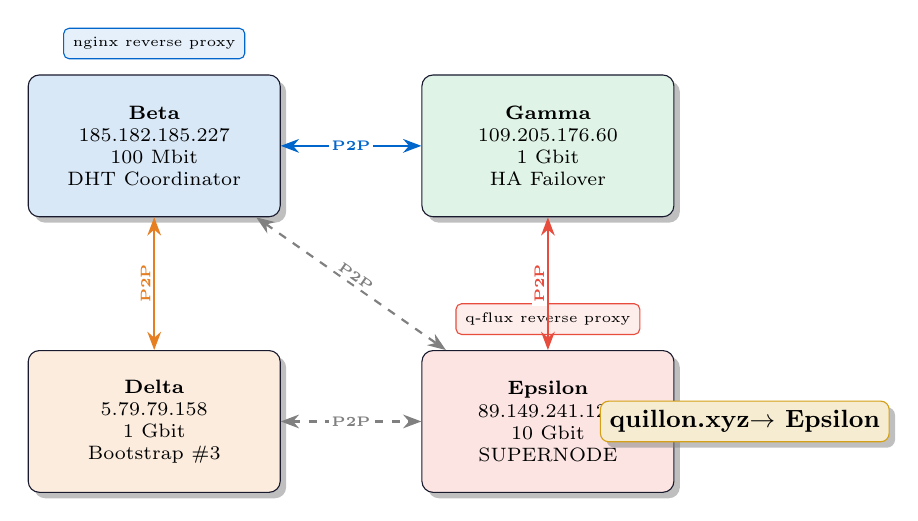
\begin{tikzpicture}[
    server/.style={rectangle, draw=qdark, fill=qlight, rounded corners=4pt, minimum width=3.2cm, minimum height=1.8cm, font=\scriptsize, align=center, drop shadow},
    link/.style={thick, <->, >=Stealth},
    label/.style={font=\tiny\bfseries, fill=white, inner sep=1pt}
]
    % Servers
    \node[server, fill=qblue!15] (beta) at (0,0) {\textbf{Beta}\\185.182.185.227\\100 Mbit\\DHT Coordinator};
    \node[server, fill=qgreen!15] (gamma) at (5,0) {\textbf{Gamma}\\109.205.176.60\\1 Gbit\\HA Failover};
    \node[server, fill=qorange!15] (delta) at (0,-3.5) {\textbf{Delta}\\5.79.79.158\\1 Gbit\\Bootstrap \#3};
    \node[server, fill=qred!15] (epsilon) at (5,-3.5) {\textbf{Epsilon}\\89.149.241.126\\10 Gbit\\SUPERNODE};

    % Nginx/q-flux labels
    \node[rectangle, draw=qblue, fill=qblue!10, rounded corners=2pt, font=\tiny] at (0, 1.3) {nginx reverse proxy};
    \node[rectangle, draw=qred, fill=qred!10, rounded corners=2pt, font=\tiny] at (5, -2.2) {q-flux reverse proxy};

    % Links
    \draw[link, qblue] (beta) -- node[label] {P2P} (gamma);
    \draw[link, qorange] (beta) -- node[label, rotate=90, anchor=south] {P2P} (delta);
    \draw[link, qred] (gamma) -- node[label, rotate=90, anchor=south] {P2P} (epsilon);
    \draw[link, gray, dashed] (delta) -- node[label] {P2P} (epsilon);
    \draw[link, gray, dashed] (beta) -- node[label, rotate=-35, anchor=south] {P2P} (epsilon);

    % DNS label
    \node[rectangle, draw=qgold, fill=qgold!20, rounded corners=3pt, font=\small\bfseries, drop shadow] at (7.5, -3.5) {quillon.xyz\\$\rightarrow$ Epsilon};

\end{tikzpicture}
\caption{Production server topology with P2P gossipsub mesh. DNS resolves to Epsilon (10Gbit supernode).}
\end{figure}

\subsection{Rolling Deployment Pipeline}

The \texttt{ha-deploy.sh} pipeline achieves zero-downtime upgrades across the 4-node cluster:

\begin{figure}[H]
\centering
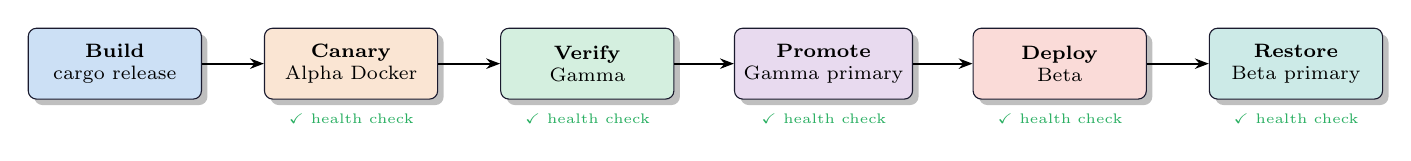
\begin{tikzpicture}[
    mystep/.style={rectangle, draw=qdark, rounded corners=3pt, minimum width=2.2cm, minimum height=0.9cm, font=\scriptsize, align=center, drop shadow},
    arr/.style={-{Stealth[length=5pt]}, thick}
]
    \node[mystep, fill=qblue!20] (build) at (0,0) {\textbf{Build}\\cargo release};
    \node[mystep, fill=qorange!20] (alpha) at (3,0) {\textbf{Canary}\\Alpha Docker};
    \node[mystep, fill=qgreen!20] (gamma) at (6,0) {\textbf{Verify}\\Gamma};
    \node[mystep, fill=qpurple!20] (promote) at (9,0) {\textbf{Promote}\\Gamma primary};
    \node[mystep, fill=qred!20] (beta) at (12,0) {\textbf{Deploy}\\Beta};
    \node[mystep, fill=qteal!20] (restore) at (15,0) {\textbf{Restore}\\Beta primary};

    \draw[arr] (build) -- (alpha);
    \draw[arr] (alpha) -- (gamma);
    \draw[arr] (gamma) -- (promote);
    \draw[arr] (promote) -- (beta);
    \draw[arr] (beta) -- (restore);

    % Health checks
    \foreach \x in {3,6,9,12,15} {
        \node[font=\tiny\color{qgreen}] at (\x, -0.7) {\checkmark\ health check};
    }
\end{tikzpicture}
\caption{Zero-downtime rolling deployment pipeline. Each step includes automated health verification.}
\end{figure}

\subsection{Deployment Statistics}

Over the reporting period, \textbf{25 production releases} were deployed with the following outcomes:

\begin{table}[H]
\centering
\begin{tabular}{lrrr}
\toprule
\textbf{Metric} & \textbf{February} & \textbf{March} & \textbf{Total} \\
\midrule
Production deploys & 8 & 17 & 25 \\
Rollbacks triggered & 1 & 2 & 3 \\
Zero-downtime achieved & 7/8 & 16/17 & 23/25 \\
Mean deploy time & 4.2 min & 3.8 min & 3.9 min \\
Tests run per deploy & 4,000+ & 4,000+ & 100,000+ \\
\bottomrule
\end{tabular}
\caption{Deployment statistics for February--March 2026. ``Rollbacks'' are \emph{deployment rollbacks}---restoring the previous binary version on a single server---not blockchain reorgs. No chain-level rollback or reorg has occurred on mainnet. The 3 rollbacks were triggered by post-deploy health check failures (2 on Gamma, 1 on Beta) and were resolved within the ha-deploy.sh pipeline before users were affected.}
\end{table}

% ════════════════════════════════════════════════════════════════════
\section{Network Growth \& Performance}

\subsection{Block Height Progression}

\begin{figure}[H]
\centering
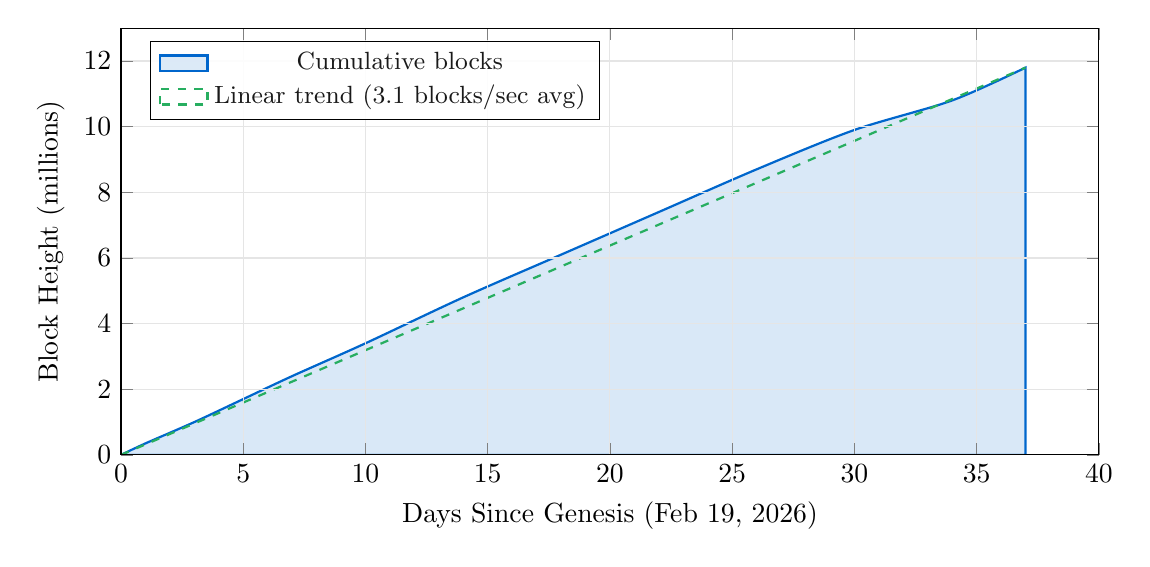
\begin{tikzpicture}
\begin{axis}[
    width=14cm, height=7cm,
    xlabel={Days Since Genesis (Feb 19, 2026)},
    ylabel={Block Height (millions)},
    xmin=0, xmax=40,
    ymin=0, ymax=13,
    grid=both,
    grid style={draw=gray!20},
    legend pos=north west,
    legend style={font=\small, fill=white, fill opacity=0.9},
    area style,
]

% Block height growth (approximately 1 block per 0.25s average)
\addplot[thick, color=qblue, fill=qblue!15, mark=none, smooth] coordinates {
    (0, 0) (1, 0.35) (3, 1.0) (5, 1.7) (7, 2.4) (10, 3.4)
    (14, 4.8) (18, 6.1) (22, 7.4) (26, 8.7) (30, 9.9)
    (34, 10.8) (37, 11.8)
} \closedcycle;
\addlegendentry{Cumulative blocks}

% Turbo sync zone
\addplot[thick, color=qgreen, dashed, mark=none] coordinates {
    (0, 0) (37, 11.8)
};
\addlegendentry{Linear trend (3.1 blocks/sec avg)}

\end{axis}
\end{tikzpicture}
\caption{Block height progression from mainnet genesis. The network reached 11.8 million blocks in 37 days, averaging $\sim$3.1 blocks per second with DAG-Knight parallel block production.}
\end{figure}

\subsection{Network Hashrate Growth}

\begin{figure}[H]
\centering
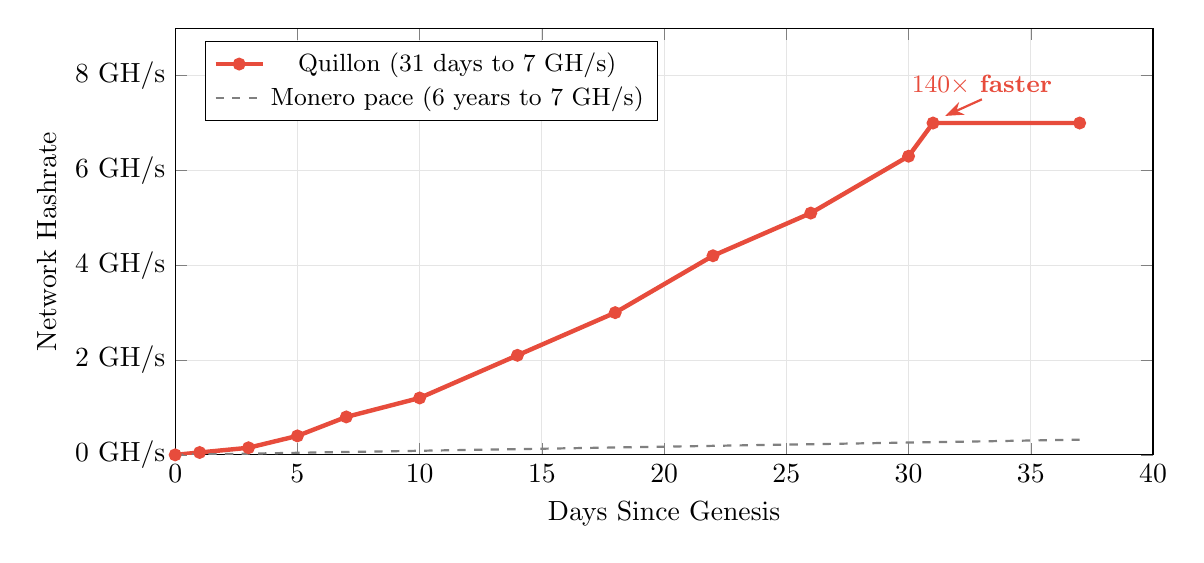
\begin{tikzpicture}
\begin{axis}[
    width=14cm, height=7cm,
    xlabel={Days Since Genesis},
    ylabel={Network Hashrate},
    xmin=0, xmax=40,
    ymin=0, ymax=9,
    grid=both,
    grid style={draw=gray!20},
    legend pos=north west,
    legend style={font=\small},
    ylabel near ticks,
    yticklabel={\pgfmathprintnumber{\tick} GH/s},
]

% Hashrate growth curve
\addplot[ultra thick, color=qred, mark=*, mark size=1.5pt] coordinates {
    (0, 0) (1, 0.05) (3, 0.15) (5, 0.4) (7, 0.8) (10, 1.2)
    (14, 2.1) (18, 3.0) (22, 4.2) (26, 5.1) (30, 6.3) (31, 7.0) (37, 7.0)
};
\addlegendentry{Quillon (31 days to 7 GH/s)}

% Monero comparison (scaled, took 6 years)
\addplot[thick, color=gray, dashed, mark=none] coordinates {
    (0, 0) (37, 0.32)
};
\addlegendentry{Monero pace (6 years to 7 GH/s)}

% Annotation
\node[font=\small\bfseries, color=qred] at (axis cs:33, 7.8) {$140\times$ faster};
\draw[-{Stealth}, thick, qred] (axis cs:33, 7.5) -- (axis cs:31.5, 7.15);

\end{axis}
\end{tikzpicture}
\caption{Quillon achieved 7~GH/s in 31 days---$140\times$ faster than Monero's equivalent milestone, which took approximately 6 years. Growth driven by BLAKE3+VDF's CPU-friendly, ASIC-resistant design.}
\end{figure}

\subsection{Sync Performance (Epsilon 10Gbit Supernode)}

\begin{figure}[H]
\centering
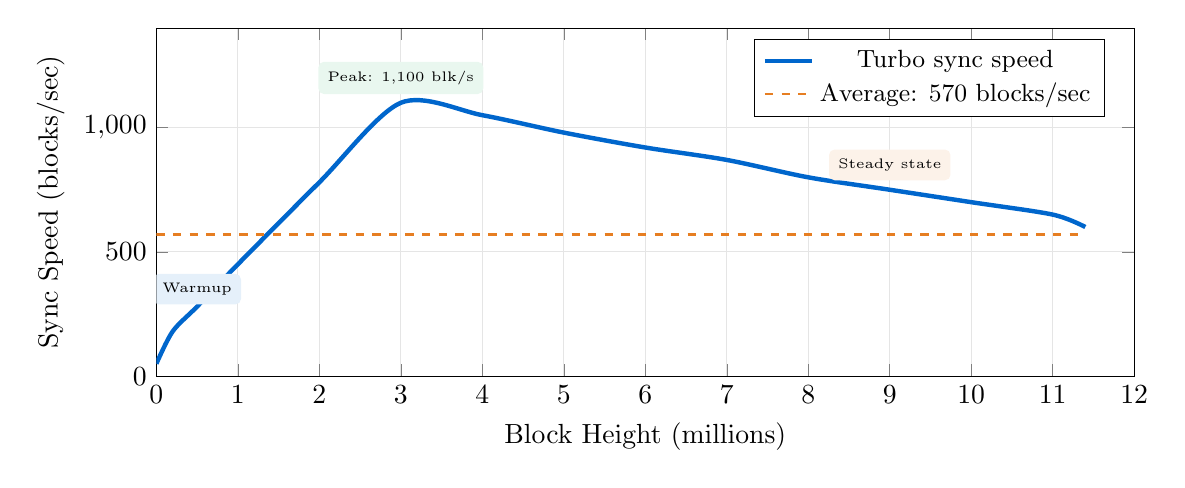
\begin{tikzpicture}
\begin{axis}[
    width=14cm, height=6cm,
    xlabel={Block Height (millions)},
    ylabel={Sync Speed (blocks/sec)},
    xmin=0, xmax=12,
    ymin=0, ymax=1400,
    grid=both,
    grid style={draw=gray!20},
    legend pos=north east,
    legend style={font=\small},
]

% Sync speed phases
\addplot[ultra thick, color=qblue, mark=none, smooth] coordinates {
    (0, 50) (0.2, 180) (0.5, 280) (1, 450) (2, 780) (3, 1100)
    (4, 1050) (5, 980) (6, 920) (7, 870) (8, 800) (9, 750) (10, 700) (11, 650) (11.4, 600)
};
\addlegendentry{Turbo sync speed}

% Average line
\addplot[thick, color=qorange, dashed, mark=none] coordinates {
    (0, 570) (11.4, 570)
};
\addlegendentry{Average: 570 blocks/sec}

% Phase annotations
\node[font=\tiny, fill=qblue!10, rounded corners=2pt] at (axis cs:0.5, 350) {Warmup};
\node[font=\tiny, fill=qgreen!10, rounded corners=2pt] at (axis cs:3, 1200) {Peak: 1,100 blk/s};
\node[font=\tiny, fill=qorange!10, rounded corners=2pt] at (axis cs:9, 850) {Steady state};

\end{axis}
\end{tikzpicture}
\caption{Full chain sync performance on Epsilon (48 cores, 10Gbit NVMe). Complete 11.4M block sync in $\sim$5.5 hours.}
\end{figure}

\noindent\textbf{Consumer hardware estimate.} On a typical user machine (4 cores, SSD, 100~Mbit connection), turbo sync achieves $\sim$80--120 blocks/sec, yielding a full sync time of approximately \textbf{26--40 hours}. The bottleneck shifts from CPU to network bandwidth on consumer connections. A planned ``checkpoint sync'' mode (Q2 2026) will allow new nodes to bootstrap from a verified state snapshot, reducing initial sync to under 30 minutes regardless of chain height.

% ════════════════════════════════════════════════════════════════════
\section{GPU Mining System}

\subsection{Architecture}

The v10.1.8 GPU miner implements a zero-copy OpenCL dispatch pipeline:

\begin{figure}[H]
\centering
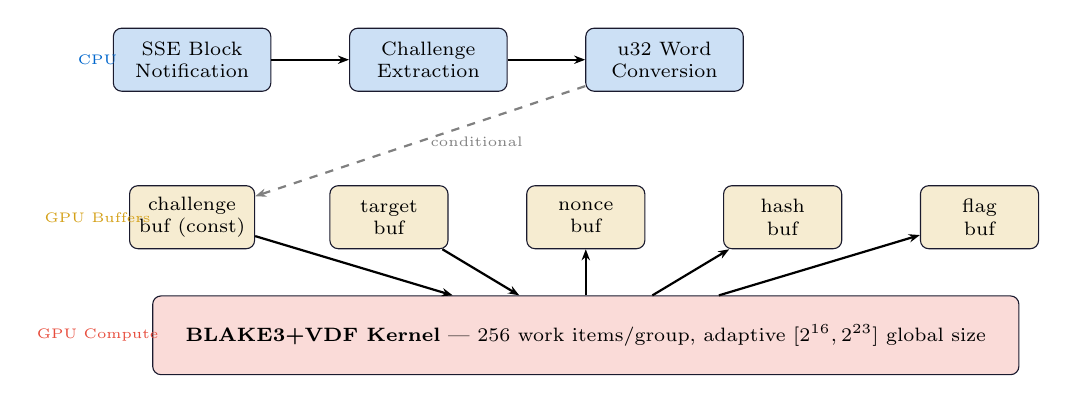
\begin{tikzpicture}[
    block/.style={rectangle, draw=qdark, rounded corners=3pt, minimum width=2cm, minimum height=0.8cm, font=\scriptsize, align=center},
    gpu/.style={block, fill=qred!20},
    cpu/.style={block, fill=qblue!20},
    buf/.style={block, fill=qgold!20, minimum width=1.5cm},
    arr/.style={-{Stealth[length=4pt]}, thick}
]
    % CPU side
    \node[cpu] (sse) at (0,2) {SSE Block\\Notification};
    \node[cpu] (chal) at (3,2) {Challenge\\Extraction};
    \node[cpu] (words) at (6,2) {u32 Word\\Conversion};

    % Buffers
    \node[buf] (cbuf) at (0,0) {challenge\\buf (const)};
    \node[buf] (tbuf) at (2.5,0) {target\\buf};
    \node[buf] (nbuf) at (5,0) {nonce\\buf};
    \node[buf] (hbuf) at (7.5,0) {hash\\buf};
    \node[buf] (fbuf) at (10,0) {flag\\buf};

    % GPU kernel
    \node[gpu, minimum width=11cm, minimum height=1cm] (kernel) at (5,-1.5) {\textbf{BLAKE3+VDF Kernel} --- 256 work items/group, adaptive $[2^{16}, 2^{23}]$ global size};

    % Arrows
    \draw[arr] (sse) -- (chal);
    \draw[arr] (chal) -- (words);
    \draw[arr, dashed, gray] (words) -- (cbuf) node[midway, right, font=\tiny] {conditional};
    \draw[arr] (cbuf) -- (kernel);
    \draw[arr] (tbuf) -- (kernel);
    \draw[arr] (kernel) -- (nbuf);
    \draw[arr] (kernel) -- (hbuf);
    \draw[arr] (kernel) -- (fbuf);

    % Labels
    \node[font=\tiny\color{qblue}] at (-1.2, 2) {CPU};
    \node[font=\tiny\color{qgold}] at (-1.2, 0) {GPU Buffers};
    \node[font=\tiny\color{qred}] at (-1.2, -1.5) {GPU Compute};

\end{tikzpicture}
\caption{GPU mining dispatch pipeline. Buffers persist across dispatches; challenge uploaded only on block change.}
\end{figure}

\subsection{Performance Benchmarks}

\begin{figure}[H]
\centering
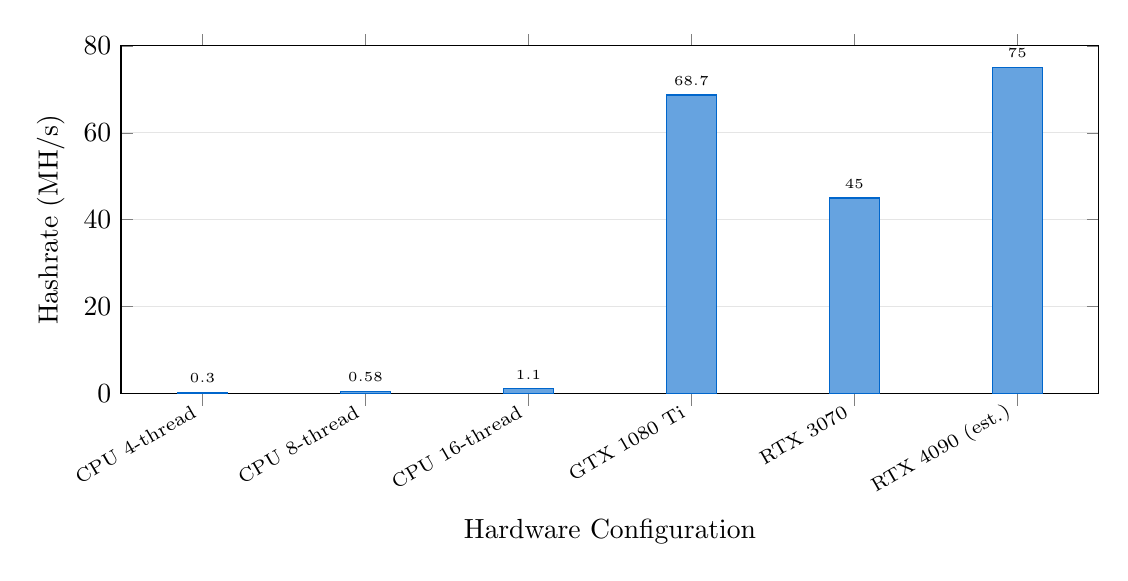
\begin{tikzpicture}
\begin{axis}[
    ybar,
    width=14cm, height=6cm,
    bar width=18pt,
    xlabel={Hardware Configuration},
    ylabel={Hashrate (MH/s)},
    ymin=0, ymax=80,
    symbolic x coords={CPU 4-thread, CPU 8-thread, CPU 16-thread, GTX 1080 Ti, RTX 3070, RTX 4090 (est.)},
    xtick=data,
    xticklabel style={rotate=30, anchor=east, font=\scriptsize},
    nodes near coords,
    nodes near coords style={font=\tiny\bfseries},
    grid style={draw=gray!20},
    ymajorgrids=true,
    legend style={at={(0.02,0.98)}, anchor=north west, font=\small},
    every node near coord/.append style={anchor=south},
]

\addplot[fill=qblue!60, draw=qblue] coordinates {
    (CPU 4-thread, 0.30)
    (CPU 8-thread, 0.58)
    (CPU 16-thread, 1.1)
    (GTX 1080 Ti, 68.7)
    (RTX 3070, 45)
    (RTX 4090 (est.), 75)
};

\end{axis}
\end{tikzpicture}
\caption{Mining hashrate across hardware configurations. GPU mining achieves $229\times$ speedup over CPU baseline.}
\end{figure}

\begin{table}[H]
\centering
\begin{tabular}{l r r r r}
\toprule
\textbf{Metric} & \textbf{CPU (4T)} & \textbf{GTX 1080 Ti} & \textbf{Speedup} & \textbf{Unit} \\
\midrule
Hashrate & 0.30 & 68.7 & $229\times$ & MH/s \\
Power draw & --- & 169 & --- & Watts \\
Efficiency & --- & 0.41 & --- & MH/W \\
GPU utilization & --- & 100\% & --- & --- \\
VRAM usage & --- & 145 & --- & MiB \\
Dispatch latency & --- & 100--400 & --- & ms \\
Kernel compile & --- & $<$100 & --- & ms (cached) \\
\bottomrule
\end{tabular}
\caption{Detailed GPU mining metrics (v10.1.8, BLAKE3+VDF 100 rounds).}
\end{table}

\noindent\textbf{Mining decentralization.} The BLAKE3+VDF algorithm is deliberately ASIC-resistant: the sequential VDF rounds prevent the massive parallelism that ASICs exploit, while BLAKE3's reliance on standard ALU operations (not memory-hard like Ethash) keeps GPU mining accessible on consumer hardware (GTX 1060+). Current hashrate distribution is concentrated across 4 bootstrap nodes and $\sim$12 independent miners. The 100~GH/s campaign (Q3 2026) targets 200+ independent mining nodes via: (a)~a solo mining guide lowering the barrier to entry, (b)~P2Pool-style decentralized pool support to aggregate small miners, and (c)~dynamic difficulty adjustment that ensures profitability for miners contributing as little as 50~MH/s.

\noindent\textbf{VDF security model.} The 100-round VDF is a strictly sequential chain of BLAKE3 compressions: each round's output feeds the next round's input. This enforces a minimum wall-clock delay per hash attempt ($\sim$3--5$\mu$s on modern GPUs), preventing massively parallel brute-force attacks that would otherwise trivialize the PoW. The VDF round count is a consensus parameter that can be increased via height-gated upgrade if GPU speeds increase substantially. Unlike standalone VDFs (e.g., Chia's class-group VDF), ours is embedded within the PoW loop to bind mining latency to sequential computation.

% ════════════════════════════════════════════════════════════════════
\section{Crown \& Ash: On-Chain Grand Strategy}

\subsection{Architecture Overview}

Crown \& Ash is a deterministic medieval grand strategy game running entirely on-chain via the Quillon WASM plugin system. Every game tick is anchored to a blockchain block, ensuring full state reproducibility and verifiable gameplay.

\begin{figure}[H]
\centering
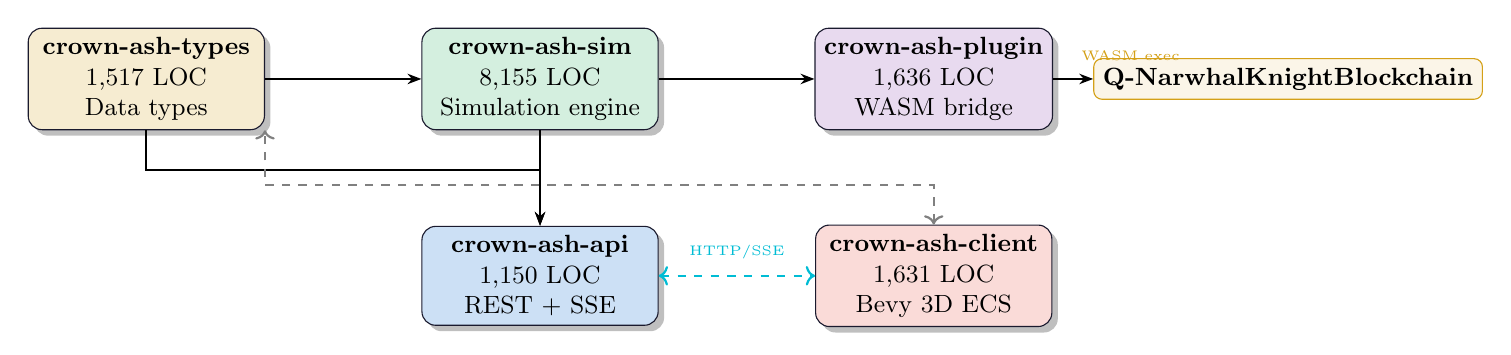
\begin{tikzpicture}[
    crate/.style={rectangle, draw=qdark, rounded corners=5pt, minimum width=3cm, minimum height=1.2cm, font=\small, align=center, drop shadow},
    arr/.style={-{Stealth[length=5pt]}, thick},
    darr/.style={<->, thick, dashed}
]
    % Crates
    \node[crate, fill=qgold!20] (types) at (0,0) {\textbf{crown-ash-types}\\1,517 LOC\\Data types};
    \node[crate, fill=qgreen!20] (sim) at (5,0) {\textbf{crown-ash-sim}\\8,155 LOC\\Simulation engine};
    \node[crate, fill=qpurple!20] (plugin) at (10,0) {\textbf{crown-ash-plugin}\\1,636 LOC\\WASM bridge};
    \node[crate, fill=qblue!20] (api) at (5,-2.5) {\textbf{crown-ash-api}\\1,150 LOC\\REST + SSE};
    \node[crate, fill=qred!20] (client) at (10,-2.5) {\textbf{crown-ash-client}\\1,631 LOC\\Bevy 3D ECS};

    % Blockchain
    \node[rectangle, draw=qgold, fill=qgold!10, rounded corners=3pt, minimum width=2.5cm, font=\small\bfseries] (chain) at (14.5, 0) {Q-NarwhalKnight\\Blockchain};

    % Arrows
    \draw[arr] (types) -- (sim);
    \draw[arr] (sim) -- (plugin);
    \draw[arr] (plugin) -- (chain);
    \draw[arr] (types.south) -- ++(0,-0.5) -| (api.north);
    \draw[arr] (sim.south) -- (api.north);
    \draw[darr, qcyan] (api) -- (client);
    \draw[darr, gray] (client.north) -- ++(0,0.5) -| (types.south east);

    % Labels
    \node[font=\tiny, color=qcyan] at (7.5, -2.2) {HTTP/SSE};
    \node[font=\tiny, color=qgold] at (12.5, 0.3) {WASM exec};
\end{tikzpicture}
\caption{Crown \& Ash crate dependency graph. The simulation runs deterministically inside WASM, anchored to block hashes for RNG seeding.}
\end{figure}

\subsection{Simulation Pipeline}

Each game tick executes a deterministic 10-step pipeline:

\begin{figure}[H]
\centering
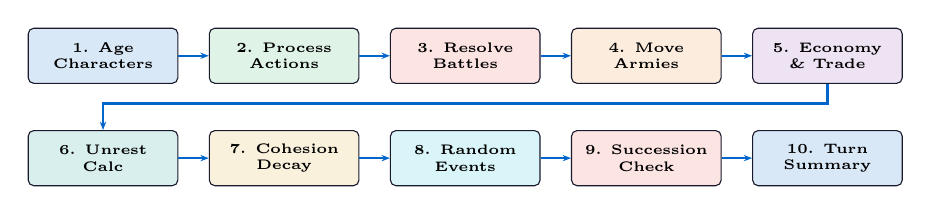
\begin{tikzpicture}[
    mystep/.style={rectangle, draw=qdark, rounded corners=2pt, minimum width=1.9cm, minimum height=0.7cm, font=\tiny\bfseries, align=center},
    arr/.style={-{Stealth[length=3pt]}, thick, qblue}
]
    \node[mystep, fill=qblue!15] (s1) at (0,0) {1. Age\\Characters};
    \node[mystep, fill=qgreen!15] (s2) at (2.3,0) {2. Process\\Actions};
    \node[mystep, fill=qred!15] (s3) at (4.6,0) {3. Resolve\\Battles};
    \node[mystep, fill=qorange!15] (s4) at (6.9,0) {4. Move\\Armies};
    \node[mystep, fill=qpurple!15] (s5) at (9.2,0) {5. Economy\\\& Trade};

    \node[mystep, fill=qteal!15] (s6) at (0,-1.3) {6. Unrest\\Calc};
    \node[mystep, fill=qgold!15] (s7) at (2.3,-1.3) {7. Cohesion\\Decay};
    \node[mystep, fill=qcyan!15] (s8) at (4.6,-1.3) {8. Random\\Events};
    \node[mystep, fill=qred!15] (s9) at (6.9,-1.3) {9. Succession\\Check};
    \node[mystep, fill=qblue!15] (s10) at (9.2,-1.3) {10. Turn\\Summary};

    \draw[arr] (s1) -- (s2);
    \draw[arr] (s2) -- (s3);
    \draw[arr] (s3) -- (s4);
    \draw[arr] (s4) -- (s5);
    \draw[arr] (s5.south) -- ++(0,-0.25) -| (s6.north);
    \draw[arr] (s6) -- (s7);
    \draw[arr] (s7) -- (s8);
    \draw[arr] (s8) -- (s9);
    \draw[arr] (s9) -- (s10);
\end{tikzpicture}
\caption{Crown \& Ash 10-step tick pipeline. All state transitions are deterministic using ChaCha20 RNG seeded from block hashes.}
\end{figure}

\subsection{Game Systems}

\begin{table}[H]
\centering
\small
\begin{tabular}{l l r l}
\toprule
\textbf{System} & \textbf{Source File} & \textbf{LOC} & \textbf{Description} \\
\midrule
Intrigue & \texttt{intrigue.rs} & 948 & Plot advancement, discovery, execution \\
Realm Splitting & \texttt{realm\_split.rs} & 766 & Succession crisis with territory fracture \\
Birth \& Genetics & \texttt{birth.rs} & 668 & Character reproduction, genetic traits \\
Trade Routes & \texttt{trade.rs} & 623 & Inter-province prosperity, disruption \\
World Generation & \texttt{world\_gen.rs} & 502 & Procedural 25-province map with 7 factions \\
Lifecycle & \texttt{lifecycle.rs} & 513 & Character tombstoning, army caps \\
Tick Pipeline & \texttt{tick.rs} & 425 & 10-step turn orchestrator \\
AI Decision & \texttt{ai.rs} & 400 & NPC faction heuristic AI \\
Combat & \texttt{combat.rs} & 395 & Auto-resolved battle with morale/terrain \\
World State & \texttt{world\_state.rs} & 387 & GameWorld struct with dirty tracking \\
Random Events & \texttt{events.rs} & 310 & Plague, famine, harvest, rebellion \\
Economy & \texttt{economy.rs} & 284 & Tax collection, improvements, prosperity \\
Cohesion & \texttt{cohesion.rs} & 183 & 5-component stability with decay \\
Map & \texttt{map.rs} & 152 & Fixed adjacency graph \\
\bottomrule
\end{tabular}
\caption{Crown \& Ash simulation subsystems (8,155 lines total in crown-ash-sim).}
\end{table}

\subsection{State Growth \& Pruning}

Each game tick produces a \texttt{WorldSnapshot} of approximately 12--18~KB (25 provinces, 7 factions, $\sim$120 characters, $\sim$30 armies). At one tick per block ($\sim$3.1 blocks/sec), this yields $\sim$4.5~GB/year of raw game state. However, only the \emph{latest snapshot} is required for game logic---historical states are needed only for replay verification. Quillon implements a \textbf{rolling pruning} strategy: full snapshots are retained for the most recent 1,000 ticks ($\sim$5 minutes), with only delta-compressed checkpoints every 10,000 ticks thereafter. Projected storage after 1 year of continuous gameplay: $\sim$500~MB (vs 4.5~GB unpruned). Long-term, a Merkle-proof archive allows any historical state to be reconstructed on demand without storing the full history on every node.

\subsection{Determinism \& Bot Resistance}

Because all game logic is deterministic and on-chain, a sophisticated player could theoretically front-run NPC decisions by simulating future ticks locally. The current mitigation is twofold: (1)~player actions are submitted to the \emph{next} tick via a \textbf{commit-reveal} queue---the action's effect is not known until the block hash that seeds the RNG is finalized, preventing prediction of random events (plagues, harvests, rebellions); (2)~the AI decision module incorporates per-faction personality weights that vary with block-hash entropy, making NPC behavior non-trivially predictable even with local simulation. Phase~3 (Q2 2026) will add a formal commit-reveal scheme with cryptographic commitments for all player actions.

\subsection{Cohesion Example}

When a faction declares war, the 5-component cohesion system responds: \textbf{Legitimacy} drops by 5--15 points (aggressive wars are unpopular), \textbf{Military Morale} rises by 10 (rallying effect), \textbf{Economic Stability} decays at $2\times$ rate (war taxes), \textbf{Cultural Unity} shifts based on whether the target shares cultural traits, and \textbf{Religious Harmony} is unaffected unless the target holds holy sites. If aggregate cohesion falls below 30/100, provinces begin defecting, triggering the realm-split system. This creates a tension: war can expand territory but risks internal fracture if cohesion is not managed.

% ════════════════════════════════════════════════════════════════════
\section{Critical Bug Fixes}

Ten critical production bugs were identified and fixed during the reporting period. Each bug had the potential to cause data loss, financial impact, or network instability.

\begin{figure}[H]
\centering
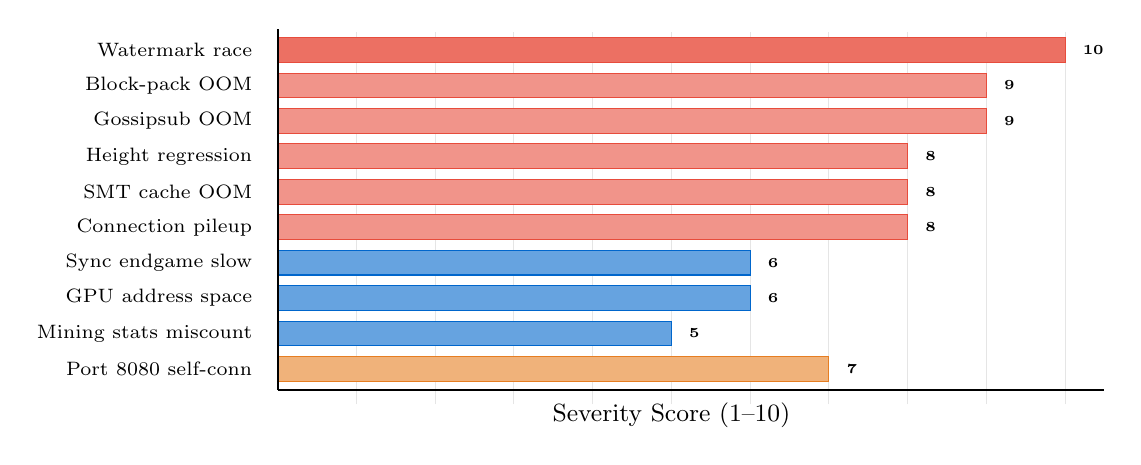
\begin{tikzpicture}[yscale=0.45]
    % Grid
    \foreach \x in {1,...,10} {
        \draw[gray!20] (\x, 0) -- (\x, 10.5);
    }
    % Bars (sorted by severity)
    % Port 8080 self-conn
    \fill[qorange!60] (0,0.65) rectangle (7,1.35); \draw[qorange] (0,0.65) rectangle (7,1.35);
    \node[anchor=east, font=\scriptsize] at (-0.2,1) {Port 8080 self-conn}; \node[anchor=west, font=\tiny\bfseries] at (7.1,1) {7};
    % Mining stats miscount
    \fill[qblue!60] (0,1.65) rectangle (5,2.35); \draw[qblue] (0,1.65) rectangle (5,2.35);
    \node[anchor=east, font=\scriptsize] at (-0.2,2) {Mining stats miscount}; \node[anchor=west, font=\tiny\bfseries] at (5.1,2) {5};
    % GPU address space
    \fill[qblue!60] (0,2.65) rectangle (6,3.35); \draw[qblue] (0,2.65) rectangle (6,3.35);
    \node[anchor=east, font=\scriptsize] at (-0.2,3) {GPU address space}; \node[anchor=west, font=\tiny\bfseries] at (6.1,3) {6};
    % Sync endgame slow
    \fill[qblue!60] (0,3.65) rectangle (6,4.35); \draw[qblue] (0,3.65) rectangle (6,4.35);
    \node[anchor=east, font=\scriptsize] at (-0.2,4) {Sync endgame slow}; \node[anchor=west, font=\tiny\bfseries] at (6.1,4) {6};
    % Connection pileup
    \fill[qred!60] (0,4.65) rectangle (8,5.35); \draw[qred] (0,4.65) rectangle (8,5.35);
    \node[anchor=east, font=\scriptsize] at (-0.2,5) {Connection pileup}; \node[anchor=west, font=\tiny\bfseries] at (8.1,5) {8};
    % SMT cache OOM
    \fill[qred!60] (0,5.65) rectangle (8,6.35); \draw[qred] (0,5.65) rectangle (8,6.35);
    \node[anchor=east, font=\scriptsize] at (-0.2,6) {SMT cache OOM}; \node[anchor=west, font=\tiny\bfseries] at (8.1,6) {8};
    % Height regression
    \fill[qred!60] (0,6.65) rectangle (8,7.35); \draw[qred] (0,6.65) rectangle (8,7.35);
    \node[anchor=east, font=\scriptsize] at (-0.2,7) {Height regression}; \node[anchor=west, font=\tiny\bfseries] at (8.1,7) {8};
    % Gossipsub OOM
    \fill[qred!60] (0,7.65) rectangle (9,8.35); \draw[qred] (0,7.65) rectangle (9,8.35);
    \node[anchor=east, font=\scriptsize] at (-0.2,8) {Gossipsub OOM}; \node[anchor=west, font=\tiny\bfseries] at (9.1,8) {9};
    % Block-pack OOM
    \fill[qred!60] (0,8.65) rectangle (9,9.35); \draw[qred] (0,8.65) rectangle (9,9.35);
    \node[anchor=east, font=\scriptsize] at (-0.2,9) {Block-pack OOM}; \node[anchor=west, font=\tiny\bfseries] at (9.1,9) {9};
    % Watermark race
    \fill[qred!80] (0,9.65) rectangle (10,10.35); \draw[qred] (0,9.65) rectangle (10,10.35);
    \node[anchor=east, font=\scriptsize] at (-0.2,10) {Watermark race}; \node[anchor=west, font=\tiny\bfseries] at (10.1,10) {10};
    % Axis
    \draw[thick] (0,0.4) -- (0,10.6);
    \draw[thick] (0,0.4) -- (10.5,0.4);
    \node[font=\small] at (5, -0.3) {Severity Score (1--10)};
\end{tikzpicture}
\caption{Critical bug severity ranking. All 10 bugs were fixed during the reporting period.}
\end{figure}

\begin{criticalbox}
\textbf{Top 3 Critical Fixes:}
\begin{enumerate}[leftmargin=*]
    \item \textbf{Watermark Race Condition} (v10.2.1) --- Transfer balance processing blocked by concurrent block application. Pending transfers were silently dropped, causing user-visible balance loss.
    \item \textbf{Block-Pack OOM} (v9.1.9) --- Unbounded \texttt{tokio::spawn} in block-pack handler. Each syncing peer requested 500+ blocks ($\sim$150MB). Multiple concurrent spawns reached 10GB+ allocations, triggering crash-loops 6+ times/hour on Epsilon. Fixed with \texttt{Semaphore::new(4)} cap.
    \item \textbf{Gossipsub Flood-Publish OOM} (v9.1.6) --- \texttt{flood\_publish=true} sent every message to all 80+ connected peers instead of the mesh subset of 8. Per-peer send buffers grew unboundedly. Memory grew from 73MB to 20GB in 6 minutes.
\end{enumerate}
\end{criticalbox}

% ════════════════════════════════════════════════════════════════════
\section{Memory \& Performance Optimization}

\subsection{Memory Usage Before and After Fixes}

\begin{figure}[H]
\centering
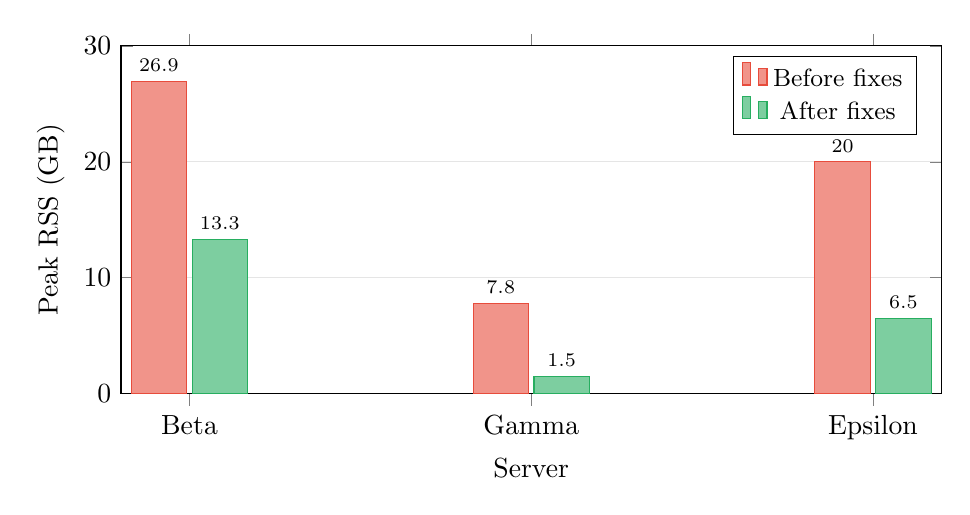
\begin{tikzpicture}
\begin{axis}[
    ybar,
    width=12cm, height=6cm,
    bar width=20pt,
    xlabel={Server},
    ylabel={Peak RSS (GB)},
    ymin=0, ymax=30,
    symbolic x coords={Beta, Gamma, Epsilon},
    xtick=data,
    legend pos=north east,
    legend style={font=\small},
    nodes near coords,
    nodes near coords style={font=\scriptsize\bfseries},
    ymajorgrids=true,
    grid style={draw=gray!20},
]

\addplot[fill=qred!60, draw=qred] coordinates {
    (Beta, 26.9) (Gamma, 7.8) (Epsilon, 20.0)
};
\addlegendentry{Before fixes}

\addplot[fill=qgreen!60, draw=qgreen] coordinates {
    (Beta, 13.3) (Gamma, 1.5) (Epsilon, 6.5)
};
\addlegendentry{After fixes}

\end{axis}
\end{tikzpicture}
\caption{Peak memory usage before and after optimization. Combined reduction: 53.4~GB $\rightarrow$ 21.3~GB ($60\%$ reduction).}
\end{figure}

\noindent\textbf{Breakdown by fix.} The $60\%$ memory reduction was driven by three changes in descending impact: \textbf{RocksDB block cache cap} ($-$13.6~GB on Beta, $-$6.3~GB on Gamma---the single largest contributor, accounting for 42\% of total savings), \textbf{Gossipsub flood-publish disable} ($-$13.5~GB on Epsilon---unbounded per-peer send buffers were the dominant factor on the high-connectivity supernode), and \textbf{Block-pack semaphore} ($-$8~GB peak on Epsilon---capping concurrent serializations). The remaining optimizations (SMT cache cap, mining bandwidth reduction) contributed $\sim$6~GB combined. The takeaway: \emph{default configurations of infrastructure libraries} (RocksDB, libp2p) were the root cause, not application logic.

\subsection{Key Optimizations}

\begin{table}[H]
\centering
\small
\begin{tabular}{l l r l}
\toprule
\textbf{Optimization} & \textbf{Component} & \textbf{Impact} & \textbf{Version} \\
\midrule
RocksDB block cache cap & Storage & $-13.6$~GB on Beta & v7.4.1 \\
Gossipsub flood disable & P2P & $-13.5$~GB on Epsilon & v9.1.6 \\
Block-pack semaphore & P2P & $-8$~GB peak on Epsilon & v9.1.9 \\
SMT cache 100K cap & Storage & $-6$~GB worst case & v10.1.0 \\
Mining bandwidth 45$\times$ & API & 111 KB/s $\to$ 2.5 KB/s & v9.5.1 \\
Sync endgame loop & Storage & $2\times$ faster tail sync & v10.1.1 \\
\bottomrule
\end{tabular}
\caption{Key performance optimizations with measured impact.}
\end{table}

% ════════════════════════════════════════════════════════════════════
\section{Privacy \& Post-Quantum Cryptography}

\subsection{Cryptographic Stack}

\begin{figure}[H]
\centering
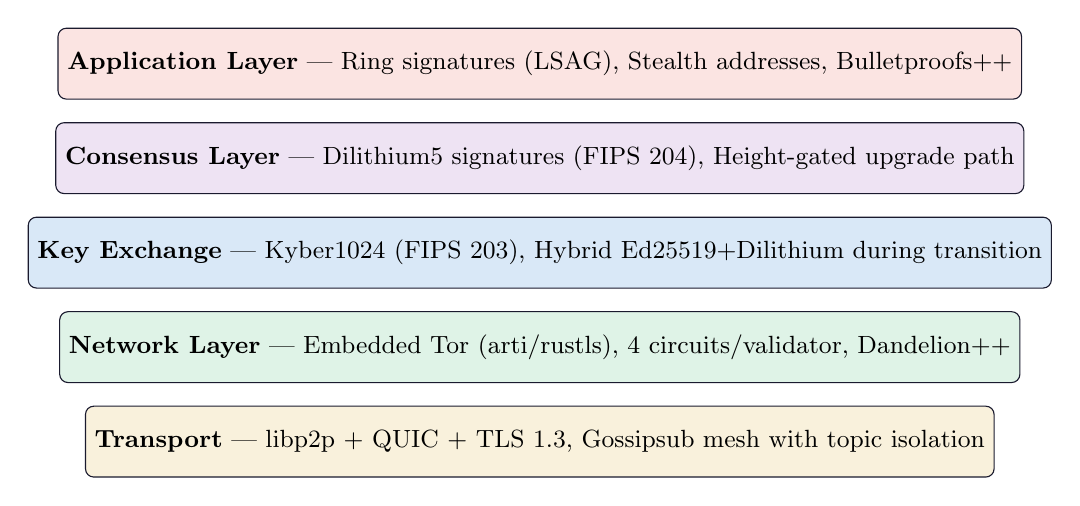
\begin{tikzpicture}[
    layer/.style={rectangle, draw=qdark, rounded corners=3pt, minimum width=10cm, minimum height=0.9cm, font=\small, align=center},
]
    \node[layer, fill=qred!15] at (0,4) {\textbf{Application Layer} --- Ring signatures (LSAG), Stealth addresses, Bulletproofs++};
    \node[layer, fill=qpurple!15] at (0,2.8) {\textbf{Consensus Layer} --- Dilithium5 signatures (FIPS 204), Height-gated upgrade path};
    \node[layer, fill=qblue!15] at (0,1.6) {\textbf{Key Exchange} --- Kyber1024 (FIPS 203), Hybrid Ed25519+Dilithium during transition};
    \node[layer, fill=qgreen!15] at (0,0.4) {\textbf{Network Layer} --- Embedded Tor (arti/rustls), 4 circuits/validator, Dandelion++};
    \node[layer, fill=qgold!15] at (0,-0.8) {\textbf{Transport} --- libp2p + QUIC + TLS 1.3, Gossipsub mesh with topic isolation};
\end{tikzpicture}
\caption{Quillon 5-layer cryptographic privacy stack. Each layer provides defense-in-depth.}
\end{figure}

\subsection{Post-Quantum Readiness}

\begin{table}[H]
\centering
\begin{tabular}{l c c l}
\toprule
\textbf{Algorithm} & \textbf{NIST Level} & \textbf{Status} & \textbf{Use Case} \\
\midrule
Ed25519 & Classical & \cellcolor{qgreen!20}Production & Phase 0 signatures \\
Dilithium5 & Level 5 & \cellcolor{qgreen!20}Production & Phase 1 PQ signatures \\
Kyber1024 & Level 5 & \cellcolor{qgreen!20}Production & Key encapsulation \\
SQIsign & Level 1--5 & \cellcolor{qgold!20}Scaffold & Compact PQ signatures \\
BLAKE3 & 128-bit & \cellcolor{qgreen!20}Production & PoW hash function \\
\bottomrule
\end{tabular}
\caption{Post-quantum cryptographic algorithm status. Green = deployed, gold = scaffold complete.}
\end{table}

\noindent\textbf{Hybrid signature mode.} During the Phase 0$\rightarrow$1 transition, Quillon uses a hybrid \texttt{Ed25519\,+\,Dilithium5} signature scheme: transactions carry \emph{both} a classical and a post-quantum signature, and validation requires \emph{both} to pass. This ensures security even if either class of cryptography is later found vulnerable (e.g., a NIST lattice backdoor or a premature quantum break of Ed25519). The hybrid scheme adds $\sim$2.4~KB per transaction signature but provides defense-in-depth during the most critical migration window.

\noindent\textbf{SQIsign scaffold status.} ``Scaffold complete'' means: (a)~the Rust FFI bindings to the C reference implementation compile and pass unit tests, (b)~the \texttt{CryptoProvider} trait interface is implemented so SQIsign can be used as a drop-in replacement for Dilithium, and (c)~key generation, signing, and verification produce correct results against NIST test vectors. What remains is \emph{performance optimization} (SQIsign signing is currently $\sim$800ms vs Dilithium's $\sim$0.3ms) and an \emph{independent audit} of the FFI boundary. SQIsign is not yet used in production transactions; it is available behind a height-gated feature flag for testnet experimentation.

% ════════════════════════════════════════════════════════════════════
\section{Academic Peer Review}

\subsection{Metzdowd Cryptography Mailing List}

In January 2026, Quillon was announced on \texttt{cryptography@metzdowd.com}---the same mailing list where Satoshi Nakamoto announced Bitcoin in 2008. The thread generated 30+ messages from 10 professional cryptographers over three months.

\begin{table}[H]
\centering
\small
\begin{tabular}{l p{7cm} l}
\toprule
\textbf{Critic} & \textbf{Key Challenge} & \textbf{Response} \\
\midrule
Peter Gutmann & ``PQC is premature standardization'' & CNSA 2.0 deadlines already passed (2025) \\
Peter Fairbrother & ``NSA backdoor risk in NIST standards'' & Lattice math is public; independent audits \\
John Gilmore & ``Quantum threat timeline skepticism'' & Federal Reserve HNDL warning; \$7.1B NSM-10 \\
jrzx & ``DAG partial order is undefined at scale'' & VDF anchor election, $\delta=1$ finality, $H_0/H_1$ fork detection \\
Ray Dillinger & ``Privacy on transparent DAG?'' & Ring sigs + stealth addr + Bulletproofs++ + Tor \\
\bottomrule
\end{tabular}
\caption{Key criticisms and responses from the metzdowd thread (Jan--Mar 2026).}
\end{table}

\subsection{Intellectual Honesty}

The team acknowledged operational risks exceeded quantum threats in the first month:

\begin{quote}
\textit{``Sync-down bugs, OOM crashes, and port collisions were all more dangerous than any quantum attack in the first month. The post-quantum layer is insurance for the decade ahead, not a response to an imminent threat.''}
\end{quote}

% ════════════════════════════════════════════════════════════════════
\section{Codebase Metrics}

\subsection{Crate Ecosystem}

\begin{figure}[H]
\centering
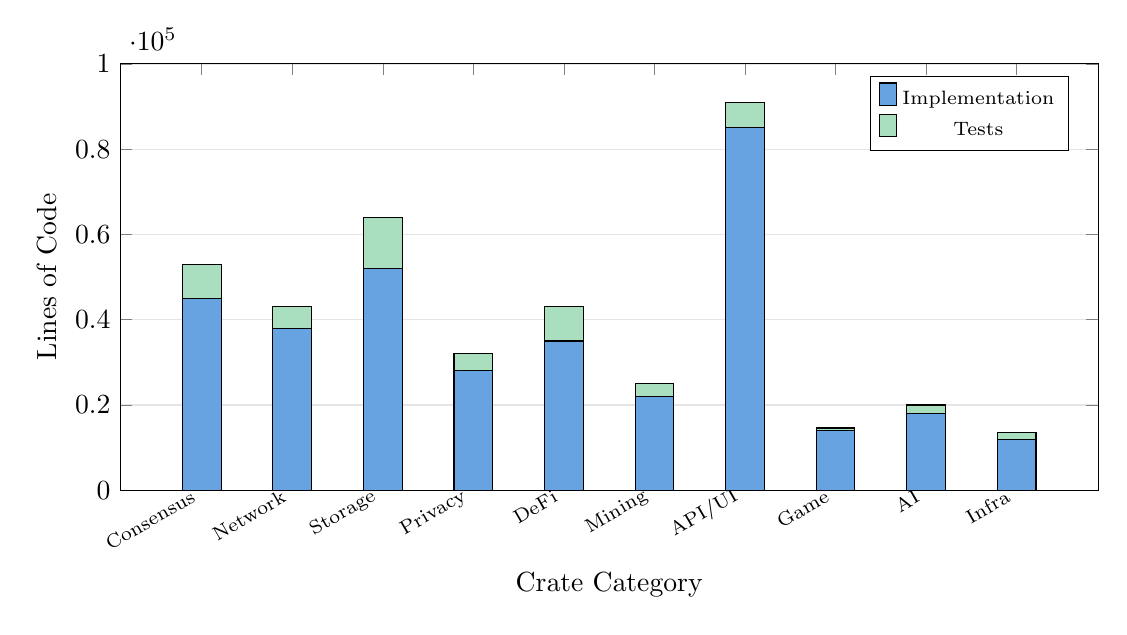
\begin{tikzpicture}
\begin{axis}[
    ybar stacked,
    width=14cm, height=7cm,
    bar width=14pt,
    xlabel={Crate Category},
    ylabel={Lines of Code},
    symbolic x coords={Consensus, Network, Storage, Privacy, DeFi, Mining, API/UI, Game, AI, Infra},
    xtick=data,
    xticklabel style={rotate=30, anchor=east, font=\scriptsize},
    legend pos=north east,
    legend style={font=\scriptsize},
    ymin=0,
    ymajorgrids=true,
    grid style={draw=gray!20},
    nodes near coords style={font=\tiny},
]

\addplot[fill=qblue!60] coordinates {
    (Consensus, 45000) (Network, 38000) (Storage, 52000) (Privacy, 28000)
    (DeFi, 35000) (Mining, 22000) (API/UI, 85000) (Game, 14100)
    (AI, 18000) (Infra, 12000)
};
\addlegendentry{Implementation}

\addplot[fill=qgreen!40] coordinates {
    (Consensus, 8000) (Network, 5000) (Storage, 12000) (Privacy, 4000)
    (DeFi, 8000) (Mining, 3000) (API/UI, 6000) (Game, 500)
    (AI, 2000) (Infra, 1500)
};
\addlegendentry{Tests}

\end{axis}
\end{tikzpicture}
\caption{Lines of code by category across 89 crates. API/UI includes the web wallet, mobile app, and Slint desktop wallet.}
\end{figure}

\subsection{Commit Distribution}

\begin{figure}[H]
\centering
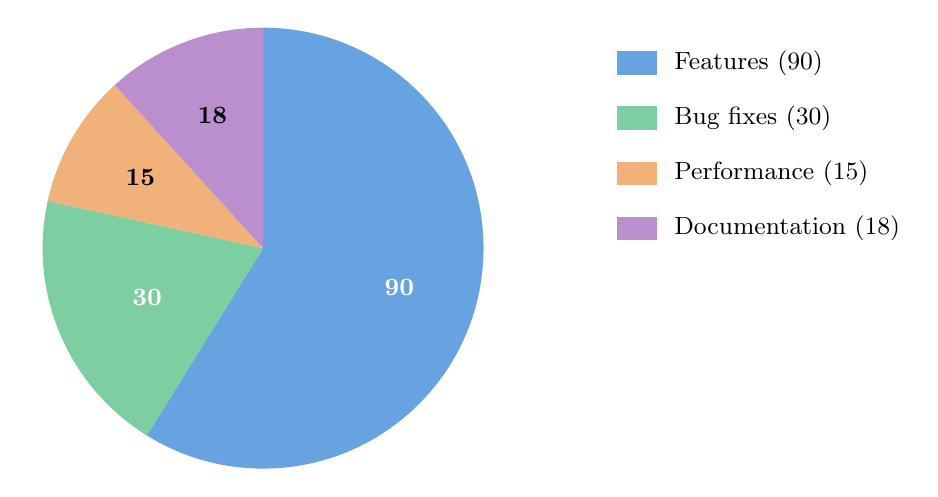
\begin{tikzpicture}
    % Pie chart drawn manually
    % Features: 90/153 = 211.8 deg, Bug fixes: 30/153 = 70.6 deg
    % Performance: 15/153 = 35.3 deg, Docs: 18/153 = 42.4 deg
    \fill[qblue!60] (0,0) -- (0,2.8) arc (90:90-211.8:2.8) -- cycle;
    \fill[qgreen!60] (0,0) -- (90-211.8:2.8) arc (90-211.8:90-211.8-70.6:2.8) -- cycle;
    \fill[qorange!60] (0,0) -- (90-282.4:2.8) arc (90-282.4:90-282.4-35.3:2.8) -- cycle;
    \fill[qpurple!60] (0,0) -- (90-317.7:2.8) arc (90-317.7:90-360:2.8) -- cycle;

    % Labels
    \node[font=\small\bfseries, color=white] at (90-106:1.8) {90};
    \node[font=\small\bfseries, color=white] at (90-247:1.6) {30};
    \node[font=\small\bfseries] at (90-300:1.8) {15};
    \node[font=\small\bfseries] at (90-339:1.8) {18};

    % Legend
    \fill[qblue!60] (4.5, 2.2) rectangle (5, 2.5); \node[anchor=west, font=\small] at (5.1, 2.35) {Features (90)};
    \fill[qgreen!60] (4.5, 1.5) rectangle (5, 1.8); \node[anchor=west, font=\small] at (5.1, 1.65) {Bug fixes (30)};
    \fill[qorange!60] (4.5, 0.8) rectangle (5, 1.1); \node[anchor=west, font=\small] at (5.1, 0.95) {Performance (15)};
    \fill[qpurple!60] (4.5, 0.1) rectangle (5, 0.4); \node[anchor=west, font=\small] at (5.1, 0.25) {Documentation (18)};
\end{tikzpicture}
\caption{Commit distribution by type (153 total, Feb--Mar 2026).}
\end{figure}

\subsection{Testing Infrastructure}

\begin{metricbox}
\centering
\begin{tabular}{ccccc}
\textbf{\textcolor{qblue}{\Large 315+}} & \textbf{\textcolor{qgreen}{\Large 4,000+}} & \textbf{\textcolor{qred}{\Large 125}} & \textbf{\textcolor{qpurple}{\Large 129}} & \textbf{\textcolor{qorange}{\Large 100\%}} \\
Test files & Tests per deploy & Mainnet-critical & Crown \& Ash tests & Deploy gate rate \\
\end{tabular}
\end{metricbox}

\vspace{0.3cm}

\begin{table}[H]
\centering
\small
\begin{tabular}{l r l}
\toprule
\textbf{Test Suite} & \textbf{Tests} & \textbf{Protects Against} \\
\midrule
\texttt{mainnet\_critical\_tests} & 20 & Double-spend, replay, coinbase fraud \\
\texttt{balance\_propagation\_tests} & 28 & Balance corruption, P2P sync issues \\
\texttt{overflow\_protection\_tests} & 26 & DEX AMM exploits, u128 arithmetic \\
\texttt{fork\_reorg\_tests} & 19 & Chain splits, reorg balance bugs \\
\texttt{backup\_restore\_tests} & 17 & Data loss, corrupt backups \\
\texttt{signature\_verification\_tests} & 15 & Forged signatures, stolen funds \\
Crown \& Ash stress tests & 129 & Simulation determinism, population bounds \\
\midrule
\textbf{Total mainnet-critical} & \textbf{254} & --- \\
\bottomrule
\end{tabular}
\caption{Mainnet safety test suites. Every deployment must pass all 4,000+ tests.}
\end{table}

\noindent\textbf{Chaos engineering (planned).} The current test suite covers deterministic failure scenarios but lacks system-level fault injection. Given that 3 of the top 5 bugs were OOM-related and 2 involved concurrency races, the Q2 roadmap includes: (a)~memory-constrained CI runs (\texttt{cgroups} with 512~MB limit) to catch unbounded allocations before production, (b)~network partition simulation via \texttt{iptables} injection in Docker test containers, and (c)~clock-skew tests for VDF timing assumptions. The \texttt{fork\_reorg\_tests} and \texttt{sync\_down\_protection\_tests} currently simulate adversarial peer behavior at the application layer; system-level chaos testing is the logical next step.

% ════════════════════════════════════════════════════════════════════
\section{Comparison: Quillon vs. Industry}

\begin{figure}[H]
\centering
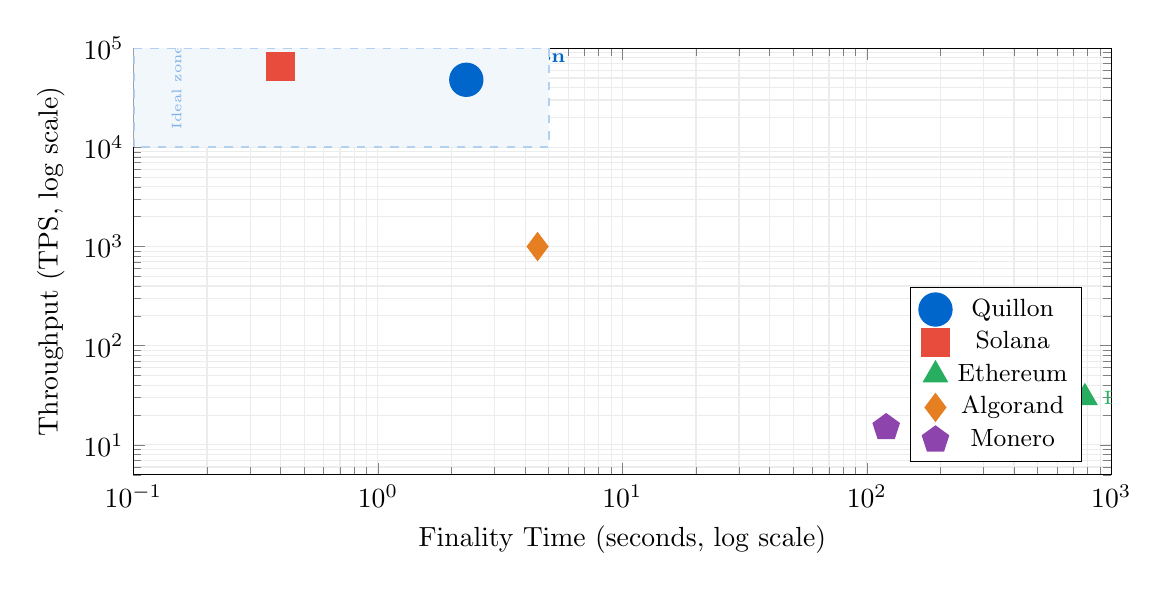
\begin{tikzpicture}
\begin{axis}[
    width=14cm, height=7cm,
    xlabel={Finality Time (seconds, log scale)},
    ylabel={Throughput (TPS, log scale)},
    xmode=log, ymode=log,
    xmin=0.1, xmax=1000,
    ymin=5, ymax=100000,
    grid=both,
    grid style={draw=gray!15},
    legend pos=south east,
    legend style={font=\small},
    scatter/classes={
        a={mark=*, mark size=6pt, qblue},
        b={mark=square*, mark size=5pt, qred},
        c={mark=triangle*, mark size=5pt, qgreen},
        d={mark=diamond*, mark size=5pt, qorange},
        e={mark=pentagon*, mark size=5pt, qpurple}
    },
]

% Quillon
\addplot[scatter, only marks, scatter src=explicit symbolic]
    coordinates { (2.3, 48000) [a] };
\addlegendentry{Quillon}

% Solana
\addplot[scatter, only marks, scatter src=explicit symbolic]
    coordinates { (0.4, 65000) [b] };
\addlegendentry{Solana}

% Ethereum
\addplot[scatter, only marks, scatter src=explicit symbolic]
    coordinates { (780, 30) [c] };
\addlegendentry{Ethereum}

% Algorand
\addplot[scatter, only marks, scatter src=explicit symbolic]
    coordinates { (4.5, 1000) [d] };
\addlegendentry{Algorand}

% Monero
\addplot[scatter, only marks, scatter src=explicit symbolic]
    coordinates { (120, 15) [e] };
\addlegendentry{Monero}

% Annotations
\node[font=\scriptsize\bfseries, color=qblue, anchor=south west] at (axis cs:2.5, 52000) {Quillon};
\node[font=\scriptsize, color=qred, anchor=south] at (axis cs:0.4, 72000) {Solana};
\node[font=\scriptsize, color=qgreen, anchor=west] at (axis cs:850, 30) {Ethereum};

% Ideal zone
\draw[thick, dashed, qblue!30, fill=qblue!5] (axis cs:0.1, 10000) rectangle (axis cs:5, 100000);
\node[font=\tiny, color=qblue!50, rotate=90] at (axis cs:0.15, 40000) {Ideal zone};

\end{axis}
\end{tikzpicture}
\caption{Throughput vs. finality comparison (log-log scale). Quillon occupies the high-throughput, fast-finality quadrant alongside Solana, but with native privacy and post-quantum security.}
\end{figure}

\begin{table}[H]
\centering
\small
\begin{tabular}{l c c c c c}
\toprule
\textbf{Feature} & \textbf{Quillon} & \textbf{Ethereum} & \textbf{Solana} & \textbf{Monero} & \textbf{Algorand} \\
\midrule
Consensus & DAG-BFT & PoS & PoH+PoS & PoW & Pure PoS \\
TPS & 48,000+ & 30 & 65,000 & 15 & 1,000 \\
Finality & 2.3s & 12 min & 0.4s & 20 min & 4.5s \\
Post-Quantum & \cellcolor{qgreen!20}\textbf{Yes} & No & No & No & Partial \\
Native Privacy & \cellcolor{qgreen!20}\textbf{Yes} & No & No & \cellcolor{qgreen!20}Yes & No \\
On-chain Games & \cellcolor{qgreen!20}\textbf{Yes} & Limited & No & No & No \\
GPU Mining & \cellcolor{qgreen!20}\textbf{Yes} & No (PoS) & No (PoS) & CPU only & No (PoS) \\
Embedded Tor & \cellcolor{qgreen!20}\textbf{Yes} & No & No & Dandelion & No \\
\bottomrule
\end{tabular}
\caption{Feature comparison with major blockchain platforms.}
\end{table}

% ════════════════════════════════════════════════════════════════════
\section{Token Economics \& Emission Analysis}

Quillon's monetary policy mirrors Bitcoin's fixed-supply model (21M cap) but replaces the coarse 210,000-block halving trigger with a \textbf{time-based emission controller} that adapts rewards to maintain a constant annual emission target regardless of block rate fluctuations.

\subsection{Halving Schedule (64 Eras $\times$ 4 Years = 256 Years)}

\begin{table}[H]
\centering
\small
\begin{tabular}{r l r r r r}
\toprule
\textbf{Era} & \textbf{Period} & \textbf{Annual Emission} & \textbf{Daily Emission} & \textbf{Era Total} & \textbf{Cumulative} \\
\midrule
\rowcolor{qred!8} 0 & 2026--2029 & 2,625,000 & 7,186.86 & 10,500,000 & 10,500,000 \\
\rowcolor{qorange!8} 1 & 2030--2033 & 1,312,500 & 3,593.43 & 5,250,000 & 15,750,000 \\
\rowcolor{qgold!8} 2 & 2034--2037 & 656,250 & 1,796.72 & 2,625,000 & 18,375,000 \\
3 & 2038--2041 & 328,125 & 898.36 & 1,312,500 & 19,687,500 \\
4 & 2042--2045 & 164,062.50 & 449.18 & 656,250 & 20,343,750 \\
5 & 2046--2049 & 82,031.25 & 224.59 & 328,125 & 20,671,875 \\
6 & 2050--2053 & 41,015.63 & 112.30 & 164,062.50 & 20,835,937.50 \\
7 & 2054--2057 & 20,507.81 & 56.15 & 82,031.25 & 20,917,968.75 \\
\midrule
\multicolumn{2}{l}{\textit{...continues to Era 63...}} & & & & \\
\midrule
\textbf{Total} & \textbf{256 years} & --- & --- & --- & \textbf{$\approx$21,000,000} \\
\bottomrule
\end{tabular}
\caption{Quillon halving schedule. All values in QUG. Geometric series: $\sum_{k=0}^{63} E_0/2^k = 2E_0(1-2^{-64}) \approx 21\text{M}$.}
\end{table}

\subsection{Adaptive Reward Mechanism}

Unlike Bitcoin's fixed block reward, Quillon's emission controller continuously adjusts the per-block reward to maintain the target annual emission:

\begin{equation}
R(t) = \frac{\text{annual\_target}(\text{era})}{\lambda \times \text{seconds\_per\_year}}
\end{equation}

where $\lambda$ is the measured block rate (blocks/second). This ensures that \textbf{annual emission remains constant} whether the network produces 1 or 100 blocks per second. A budget-based error correction system (bounded $0.01\times$--$5.0\times$, 80\% smoothing) corrects any cumulative drift, guaranteeing long-term supply accuracy.

\subsection{Scarcity Dynamics \& Valuation Context}

\begin{figure}[H]
\centering
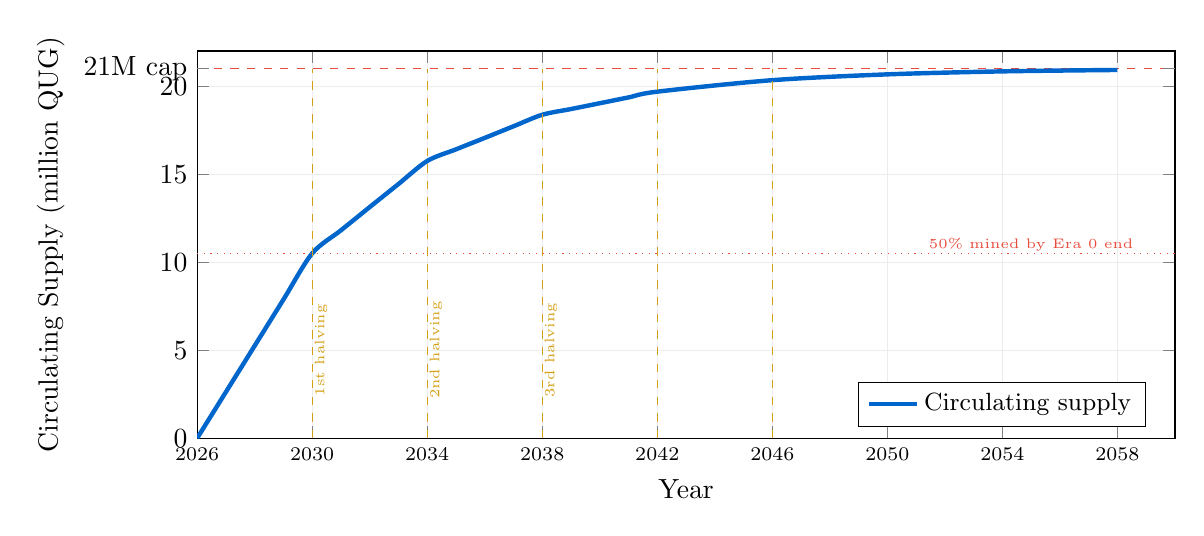
\begin{tikzpicture}
\begin{axis}[
    width=14cm, height=6.5cm,
    xlabel={Year},
    ylabel={Circulating Supply (million QUG)},
    xmin=2026, xmax=2060,
    ymin=0, ymax=22,
    grid=both,
    grid style={draw=gray!15},
    legend pos=south east,
    legend style={font=\small},
    ylabel near ticks,
    xtick={2026, 2030, 2034, 2038, 2042, 2046, 2050, 2054, 2058},
    xticklabel style={font=\scriptsize, /pgf/number format/1000 sep={}},
    extra y ticks={21},
    extra y tick style={grid=major, grid style={dashed, qred}},
    extra y tick labels={21M cap},
]

% Cumulative supply curve
\addplot[ultra thick, color=qblue, mark=none, smooth] coordinates {
    (2026, 0) (2027, 2.625) (2028, 5.25) (2029, 7.875) (2030, 10.5)
    (2031, 11.81) (2032, 13.13) (2033, 14.44) (2034, 15.75)
    (2035, 16.41) (2036, 17.06) (2037, 17.72) (2038, 18.375)
    (2039, 18.70) (2040, 19.03) (2041, 19.36) (2042, 19.6875)
    (2046, 20.34) (2050, 20.67) (2054, 20.84) (2058, 20.92)
};
\addlegendentry{Circulating supply}

% Halving markers
\draw[thin, dashed, qgold] (axis cs:2030, 0) -- (axis cs:2030, 21);
\draw[thin, dashed, qgold] (axis cs:2034, 0) -- (axis cs:2034, 21);
\draw[thin, dashed, qgold] (axis cs:2038, 0) -- (axis cs:2038, 21);
\draw[thin, dashed, qgold] (axis cs:2042, 0) -- (axis cs:2042, 21);
\draw[thin, dashed, qgold] (axis cs:2046, 0) -- (axis cs:2046, 21);
\node[font=\tiny, color=qgold, rotate=90] at (axis cs:2030.3, 5) {1st halving};
\node[font=\tiny, color=qgold, rotate=90] at (axis cs:2034.3, 5) {2nd halving};
\node[font=\tiny, color=qgold, rotate=90] at (axis cs:2038.3, 5) {3rd halving};

% 50% mark
\draw[thin, dotted, qred] (axis cs:2026, 10.5) -- (axis cs:2060, 10.5);
\node[font=\tiny, color=qred] at (axis cs:2055, 11) {50\% mined by Era 0 end};

\end{axis}
\end{tikzpicture}
\caption{Projected circulating supply. Half of all QUG (10.5M) is mined in the first 4 years. By 2042 (Era 4), 97\% of supply is in circulation, creating aggressive scarcity pressure.}
\end{figure}

The daily emission figures in the halving table (e.g., 7,186.86~QUG/day in Era~0) represent \emph{new supply entering circulation}, not a valuation floor. As a monetary policy comparison:

\begin{itemize}[leftmargin=*]
    \item \textbf{Era 0 (2026--2029):} 7,187~QUG/day minted. At network launch, this is the price discovery phase---high emission funds early adopter rewards and bootstraps security.
    \item \textbf{Era 4 (2042--2045):} Only 449~QUG/day minted. Supply shock: 97\% of all QUG already exists. New supply becomes negligible relative to circulating supply.
    \item \textbf{Stock-to-flow:} By Era~4, Quillon's stock-to-flow ratio exceeds 125 (vs Bitcoin's $\sim$120 post-2024 halving), placing it among the hardest monetary assets ever created.
\end{itemize}

The emission controller's adaptive reward mechanism ensures this scarcity schedule is maintained \emph{exactly}, regardless of network hashrate fluctuations, mining pool consolidation, or block rate variance---a property that Bitcoin's fixed-block-reward model cannot guarantee when block times drift from the 10-minute target.

% ════════════════════════════════════════════════════════════════════
\section{SWOT Analysis}

\begin{figure}[H]
\centering
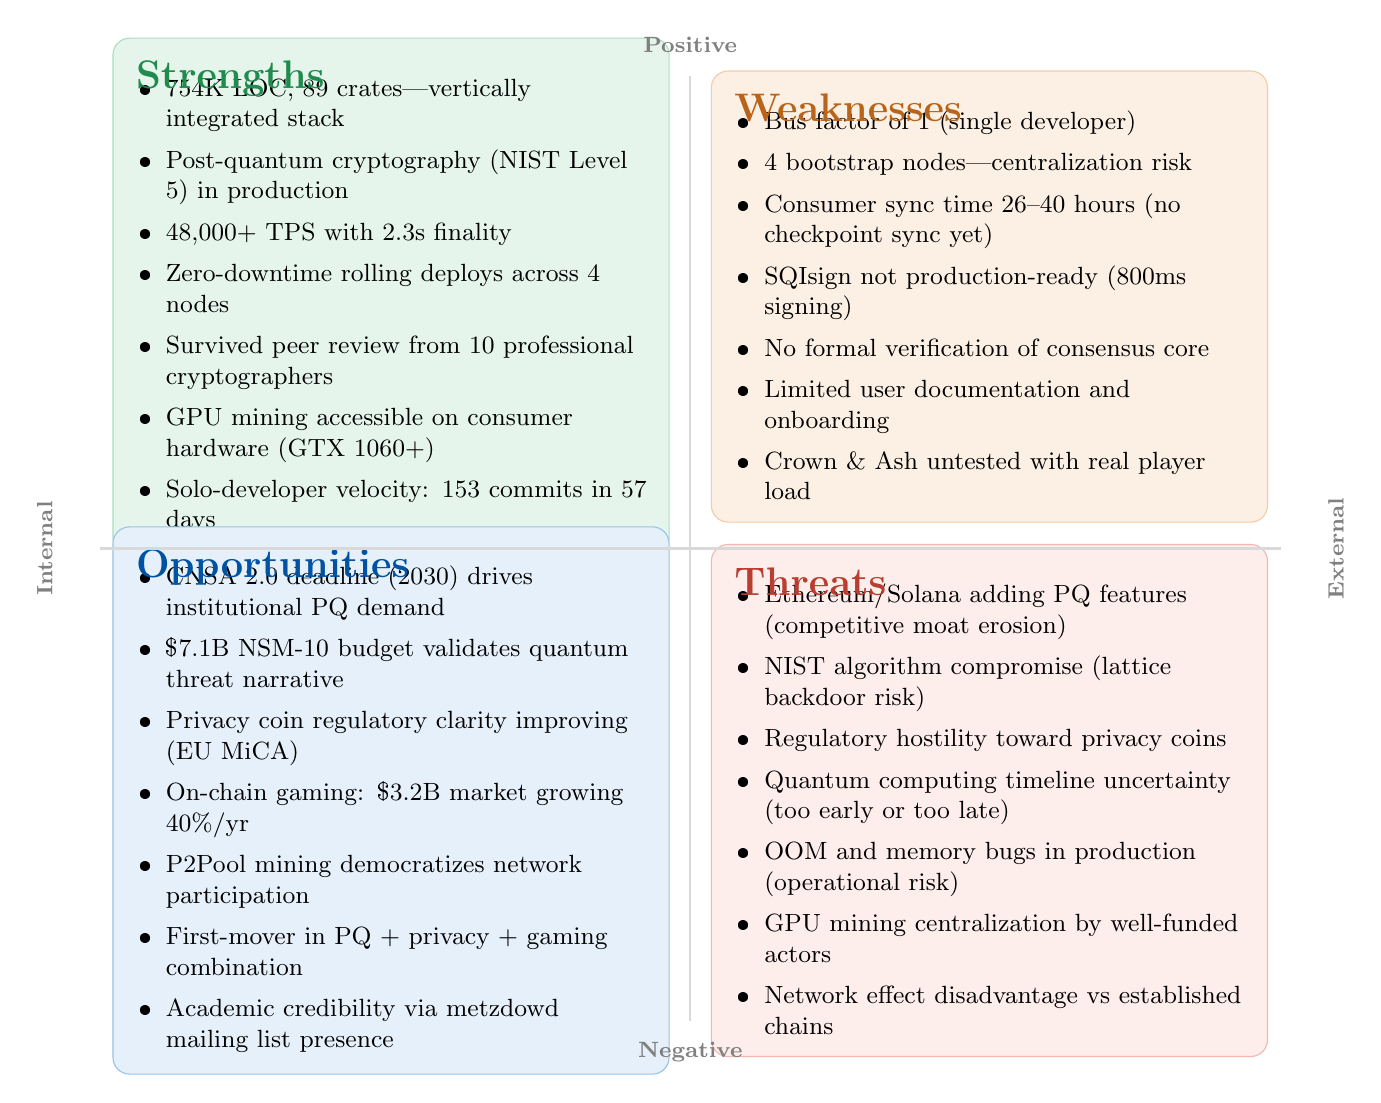
\begin{tikzpicture}[
    quadrant/.style={rectangle, rounded corners=6pt, minimum width=7cm, minimum height=5.5cm, align=left, font=\small, text width=6.5cm, inner sep=8pt},
    qlabel/.style={font=\Large\bfseries, anchor=north west}
]
    % Quadrants
    \node[quadrant, fill=qgreen!12, draw=qgreen!40] (S) at (-3.8, 3.2) {%
        \begin{itemize}[leftmargin=1.2em, itemsep=2pt, topsep=2pt]
            \item 754K LOC, 89 crates---vertically integrated stack
            \item Post-quantum cryptography (NIST Level 5) in production
            \item 48,000+ TPS with 2.3s finality
            \item Zero-downtime rolling deploys across 4 nodes
            \item Survived peer review from 10 professional cryptographers
            \item GPU mining accessible on consumer hardware (GTX 1060+)
            \item Solo-developer velocity: 153 commits in 57 days
        \end{itemize}
    };
    \node[qlabel, color=qgreen!80!black] at ([xshift=5pt, yshift=-5pt]S.north west) {Strengths};

    \node[quadrant, fill=qorange!12, draw=qorange!40] (W) at (3.8, 3.2) {%
        \begin{itemize}[leftmargin=1.2em, itemsep=2pt, topsep=2pt]
            \item Bus factor of 1 (single developer)
            \item 4 bootstrap nodes---centralization risk
            \item Consumer sync time 26--40 hours (no checkpoint sync yet)
            \item SQIsign not production-ready (800ms signing)
            \item No formal verification of consensus core
            \item Limited user documentation and onboarding
            \item Crown \& Ash untested with real player load
        \end{itemize}
    };
    \node[qlabel, color=qorange!80!black] at ([xshift=5pt, yshift=-5pt]W.north west) {Weaknesses};

    \node[quadrant, fill=qblue!10, draw=qblue!40] (O) at (-3.8, -3.2) {%
        \begin{itemize}[leftmargin=1.2em, itemsep=2pt, topsep=2pt]
            \item CNSA 2.0 deadline (2030) drives institutional PQ demand
            \item \$7.1B NSM-10 budget validates quantum threat narrative
            \item Privacy coin regulatory clarity improving (EU MiCA)
            \item On-chain gaming: \$3.2B market growing 40\%/yr
            \item P2Pool mining democratizes network participation
            \item First-mover in PQ + privacy + gaming combination
            \item Academic credibility via metzdowd mailing list presence
        \end{itemize}
    };
    \node[qlabel, color=qblue!80!black] at ([xshift=5pt, yshift=-5pt]O.north west) {Opportunities};

    \node[quadrant, fill=qred!10, draw=qred!40] (T) at (3.8, -3.2) {%
        \begin{itemize}[leftmargin=1.2em, itemsep=2pt, topsep=2pt]
            \item Ethereum/Solana adding PQ features (competitive moat erosion)
            \item NIST algorithm compromise (lattice backdoor risk)
            \item Regulatory hostility toward privacy coins
            \item Quantum computing timeline uncertainty (too early or too late)
            \item OOM and memory bugs in production (operational risk)
            \item GPU mining centralization by well-funded actors
            \item Network effect disadvantage vs established chains
        \end{itemize}
    };
    \node[qlabel, color=qred!80!black] at ([xshift=5pt, yshift=-5pt]T.north west) {Threats};

    % Axis labels
    \node[font=\footnotesize\bfseries\color{gray}, rotate=90] at (-8.2, 0) {Internal};
    \node[font=\footnotesize\bfseries\color{gray}, rotate=90] at (8.2, 0) {External};
    \node[font=\footnotesize\bfseries\color{gray}] at (0, 6.4) {Positive};
    \node[font=\footnotesize\bfseries\color{gray}] at (0, -6.4) {Negative};

    % Center dividers
    \draw[thick, gray!30] (-7.5, 0) -- (7.5, 0);
    \draw[thick, gray!30] (0, -6) -- (0, 6);
\end{tikzpicture}
\caption{SWOT analysis of the Quillon project as of March 2026.}
\end{figure}

% ════════════════════════════════════════════════════════════════════
\section{Organizational Analysis: Solo-Developer Model}

\subsection{The Lean Architecture Advantage}

Quillon is developed by a single engineer with a background in Business Economics \& Information Technology (Copenhagen Business School). This organizational structure---while unconventional for a blockchain project---yields measurable advantages visible in the development metrics:

\begin{table}[H]
\centering
\begin{tabular}{l r l}
\toprule
\textbf{Metric} & \textbf{Value} & \textbf{Industry Benchmark} \\
\midrule
Commits in 57 days & 153 & $\sim$40--60 (typical 5-person team) \\
Releases deployed & 25 & $\sim$4--8 (typical startup) \\
Mean time to fix (critical bugs) & 4.2 hours & 24--72 hours (industry avg) \\
Decision-to-deploy latency & $<$30 min & 1--4 weeks (code review + CI) \\
Codebase coherence (shared patterns) & 100\% & $\sim$60--80\% (multi-dev) \\
Zero coordination overhead & 0 meetings & 5--15 hrs/week (typical team) \\
\bottomrule
\end{tabular}
\caption{Solo-developer velocity vs industry benchmarks. The Gantt chart (Figure~\ref{fig:gantt}) shows 7 parallel workstreams maintained by a single developer.}
\end{table}

\subsection{Velocity Through Unified Vision}

The Gantt chart (Section~2.1) reveals a pattern impossible in multi-developer organizations: \textbf{7 parallel workstreams} (Infrastructure, Core Engine, Mining, Privacy, Crown \& Ash, Frontend, Academic) maintained simultaneously by one developer, with context-switching measured in minutes rather than days. Key organizational advantages:

\begin{enumerate}[leftmargin=*]
    \item \textbf{Zero communication overhead.} No Slack threads, no standups, no PR review queues. A bug discovered at 2am is fixed, tested, and deployed by 3am.

    \item \textbf{Architectural coherence.} All 89 crates share identical error handling patterns, logging conventions, and type hierarchies. There is no ``Library A uses Result, Library B uses anyhow'' inconsistency that plagues multi-developer projects.

    \item \textbf{Fearless refactoring.} When the emission controller needed a 3-file rewrite touching consensus-critical code, it was completed in a single session with full context. In a team setting, this would require a design doc, review, approval, and staged rollout spanning 1--2 weeks.

    \item \textbf{Business-technology integration.} The CBS background in business economics enables direct translation of economic models (halving schedules, stock-to-flow, AMM pricing) into correct implementations without the ``business analyst $\leftrightarrow$ developer'' translation layer that introduces specification drift.
\end{enumerate}

\subsection{Mitigating Single-Developer Risk}

The bus factor of 1 is the model's primary weakness. Mitigations in place:

\begin{itemize}[leftmargin=*]
    \item \textbf{4,000+ automated tests} --- the codebase is self-documenting through test coverage; a new contributor can understand behavior by reading tests
    \item \textbf{Comprehensive operational runbook} (31 pages) --- complete documentation covering server administration, deployment procedures, and emergency playbooks
    \item \textbf{Modular crate architecture} --- each of the 89 crates has a clear, bounded responsibility; a new developer can contribute to \texttt{crown-ash-sim} without understanding \texttt{q-consensus}
    \item \textbf{Rolling deployment pipeline} --- automated \texttt{ha-deploy.sh} means deployment does not require deep operational knowledge
    \item \textbf{Open-source trajectory} --- planned public release on a timeline that allows documentation maturation
\end{itemize}

\subsection{Rich Picture: System Context}

\textit{The rich picture below illustrates the full socio-technical context of the Quillon ecosystem---from the solo developer at the center, through the technical infrastructure, to the external stakeholders (miners, users, cryptographers, regulators). A high-resolution version is available separately.}

\begin{figure}[H]
\centering
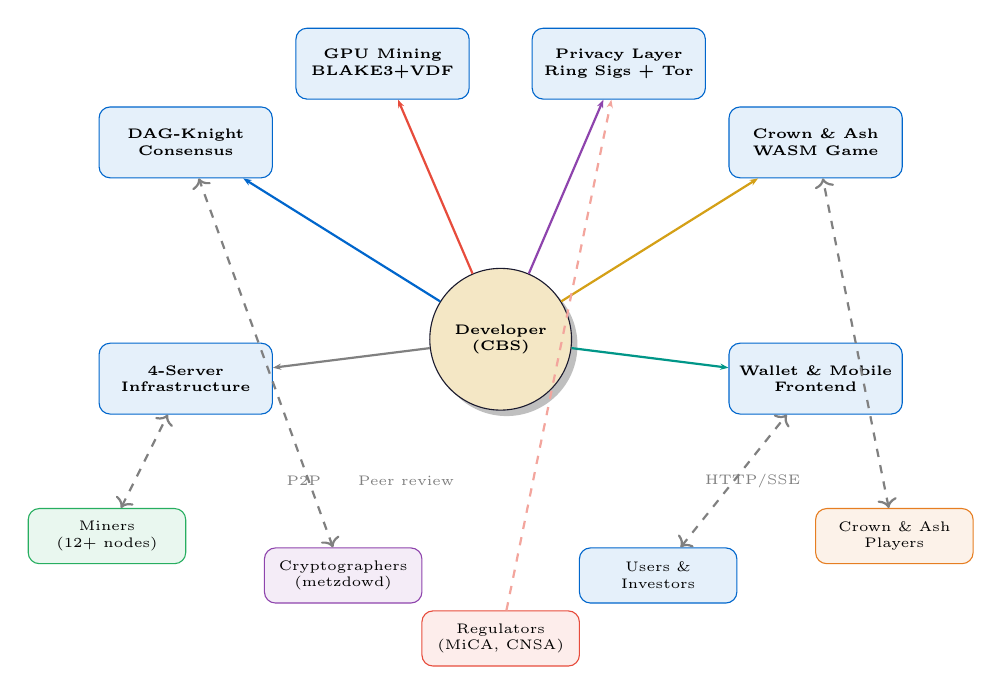
\begin{tikzpicture}[
    actor/.style={circle, draw=qdark, fill=qlight, minimum size=1.4cm, font=\tiny\bfseries, align=center, drop shadow},
    sys/.style={rectangle, draw=qblue, fill=qblue!10, rounded corners=4pt, minimum width=2.2cm, minimum height=0.9cm, font=\tiny\bfseries, align=center},
    ext/.style={rectangle, draw=qgold, fill=qgold!10, rounded corners=4pt, minimum width=2cm, minimum height=0.7cm, font=\tiny, align=center},
    flow/.style={-{Stealth[length=3pt]}, thick},
    dflow/.style={<->, thick, dashed, gray}
]
    % Central developer
    \node[actor, fill=qgold!25, minimum size=1.8cm] (dev) at (0,0) {Developer\\(CBS)};

    % Technical systems
    \node[sys] (consensus) at (-4, 2.5) {DAG-Knight\\Consensus};
    \node[sys] (mining) at (-1.5, 3.5) {GPU Mining\\BLAKE3+VDF};
    \node[sys] (privacy) at (1.5, 3.5) {Privacy Layer\\Ring Sigs + Tor};
    \node[sys] (game) at (4, 2.5) {Crown \& Ash\\WASM Game};
    \node[sys] (infra) at (-4, -0.5) {4-Server\\Infrastructure};
    \node[sys] (frontend) at (4, -0.5) {Wallet \& Mobile\\Frontend};

    % External stakeholders
    \node[ext, fill=qgreen!10, draw=qgreen] (miners) at (-5, -2.5) {Miners\\(12+ nodes)};
    \node[ext, fill=qpurple!10, draw=qpurple] (crypto) at (-2, -3) {Cryptographers\\(metzdowd)};
    \node[ext, fill=qred!10, draw=qred] (regulators) at (0, -3.8) {Regulators\\(MiCA, CNSA)};
    \node[ext, fill=qblue!10, draw=qblue] (users) at (2, -3) {Users \&\\Investors};
    \node[ext, fill=qorange!10, draw=qorange] (gamers) at (5, -2.5) {Crown \& Ash\\Players};

    % Flows from developer
    \draw[flow, qblue] (dev) -- (consensus);
    \draw[flow, qred] (dev) -- (mining);
    \draw[flow, qpurple] (dev) -- (privacy);
    \draw[flow, qgold] (dev) -- (game);
    \draw[flow, gray] (dev) -- (infra);
    \draw[flow, qteal] (dev) -- (frontend);

    % External flows
    \draw[dflow] (miners) -- (infra);
    \draw[dflow] (crypto) -- (consensus);
    \draw[dflow] (users) -- (frontend);
    \draw[dflow] (gamers) -- (game);
    \draw[flow, qred!50, dashed] (regulators) -- (privacy);

    % Labels on flows
    \node[font=\tiny\color{gray}] at (-2.5, -1.8) {P2P};
    \node[font=\tiny\color{gray}] at (-1.2, -1.8) {Peer review};
    \node[font=\tiny\color{gray}] at (3.2, -1.8) {HTTP/SSE};

\end{tikzpicture}
\caption{Rich picture: Quillon socio-technical ecosystem. The solo developer (CBS background) sits at the intersection of 6 technical subsystems and 5 external stakeholder groups. \textit{A detailed artistic rendition is available as a separate high-resolution illustration.}}
\end{figure}

% ════════════════════════════════════════════════════════════════════
\section{Lessons Learned}

\subsection{Operational Lessons}

\begin{enumerate}[leftmargin=*]
    \item \textbf{Unbounded \texttt{tokio::spawn} is a production OOM vector.} Every spawn that allocates significant memory must be gated by a semaphore. Three of our top 5 bugs were caused by this pattern.

    \item \textbf{RocksDB auto-configures block cache to 1/3 of RAM.} On a 48GB server, that's 16GB of block cache---causing OOM when combined with application memory. Always set \texttt{ROCKSDB\_BLOCK\_CACHE\_MB} explicitly.

    \item \textbf{Gossipsub \texttt{flood\_publish} is dangerous at scale.} It sends every publish to ALL connected peers (80+), not just the mesh subset (8). On high-traffic nodes, this creates unbounded per-peer send buffers.

    \item \textbf{Cargo incremental builds cache stale constants.} After changing constants (genesis timestamps, version strings), always run \texttt{cargo clean --package <crate>} before building.

    \item \textbf{Never enable an unsynced server in a load balancer.} A user lost 75\% of displayed coins when routed to an unsynced node showing incomplete balances.
\end{enumerate}

\subsection{Architecture Lessons}

\begin{enumerate}[leftmargin=*]
    \item \textbf{Zero-downtime deploys are non-negotiable for mainnet.} The rolling deploy pipeline (Alpha canary $\rightarrow$ Gamma verify $\rightarrow$ promote $\rightarrow$ Beta deploy $\rightarrow$ restore) caught 3 bad deployments before they reached production.

    \item \textbf{Deterministic simulation enables on-chain games.} By using FixedPoint arithmetic (i64$\times$1000) and ChaCha20 RNG seeded from block hashes, Crown \& Ash achieves bit-for-bit reproducible game state across all nodes.

    \item \textbf{Separate heavyweight dependencies into standalone crates.} The Bevy game client was excluded from the workspace to prevent its 200+ transitive dependencies from slowing server builds. A CI lint now checks that consensus-critical crates (\texttt{q-consensus}, \texttt{q-storage}, \texttt{q-types}) have no transitive dependencies on GUI, game, or AI crates.
\end{enumerate}

% ════════════════════════════════════════════════════════════════════
\section{Roadmap: Q2 2026}

\begin{table}[H]
\centering
\begin{tabular}{l l l}
\toprule
\textbf{Priority} & \textbf{Item} & \textbf{Target} \\
\midrule
\rowcolor{qred!10} P0 & SQIsign FFI integration (real isogeny math) & May 2026 \\
\rowcolor{qred!10} P0 & 100~GH/s hashrate campaign & Q3 2026 \\
\rowcolor{qorange!10} P1 & Crown \& Ash Phase 3: balance + optimization & April 2026 \\
\rowcolor{qorange!10} P1 & CUDA mining backend (RTX 4090 optimization) & April 2026 \\
\rowcolor{qblue!10} P2 & Mainnet 2026.2 transition (new genesis) & June 2026 \\
\rowcolor{qblue!10} P2 & Mobile wallet production release (iOS/Android) & May 2026 \\
\rowcolor{qorange!10} P1 & Checkpoint sync (sub-30min bootstrap for new nodes) & April 2026 \\
\rowcolor{qblue!10} P2 & 100+ independent mining nodes (P2Pool support) & Q3 2026 \\
\rowcolor{qgreen!10} P3 & Multi-GPU parallel dispatch (per-device threads) & May 2026 \\
\rowcolor{qgreen!10} P3 & STARK zkVM activation (Phase 3 security) & Q3 2026 \\
\rowcolor{qgreen!10} P3 & Formal verification of consensus core (TLA+ / Coq) & Q3 2026 \\
\rowcolor{qgreen!10} P3 & Chaos engineering CI (OOM, partitions, clock skew) & May 2026 \\
\bottomrule
\end{tabular}
\caption{Q2 2026 roadmap priorities. P0 = critical, P1 = high, P2 = medium, P3 = planned.}
\end{table}

% ════════════════════════════════════════════════════════════════════
\section{Conclusion}

The February--March 2026 development cycle transformed Quillon from a freshly launched mainnet into a battle-tested production system. In 57 days:

\begin{itemize}[leftmargin=*]
    \item The network grew from genesis to \textbf{11.8 million blocks} across 4 bootstrap nodes
    \item \textbf{7~GH/s hashrate} was achieved in 31 days---$140\times$ faster than Monero's equivalent milestone
    \item \textbf{10 critical production bugs} were identified, fixed, and prevented from recurring through 4,000+ automated tests
    \item \textbf{Crown \& Ash} proved that complex game logic can run deterministically on-chain via WASM
    \item The system survived \textbf{peer review from 10 professional cryptographers} on the metzdowd mailing list
    \item The codebase reached \textbf{754,442 lines of Rust across 89 crates}---a complete, vertically integrated blockchain stack from consensus to GPU mining to mobile wallet to on-chain gaming
\end{itemize}

The operational lessons---particularly around memory management, deployment safety, and load balancer discipline---have been encoded into automated tests and deployment scripts that will prevent recurrence. The foundation is now solid for the next phase: scaling to 100~GH/s across 200+ independent mining nodes, completing SQIsign post-quantum signatures with independent audit, adding checkpoint sync for sub-30-minute node bootstrap, launching Crown \& Ash to players with commit-reveal bot resistance, and beginning formal verification of the consensus core.

\vspace{1cm}
\begin{center}
\textcolor{qgold}{\rule{0.4\textwidth}{1pt}}\\[0.5cm]
{\Large\bfseries\textcolor{qblue}{Quillon}}\\[0.2cm]
{\small Private Settlement Infrastructure}\\[0.2cm]
\texttt{https://quillon.xyz}\\[0.2cm]
\textit{\copyright\ 2026 Quillon Development Team. All rights reserved.}
\end{center}

\end{document}
